\documentclass{beamer}

\usetheme{simple}

\usepackage{lmodern}
\usepackage[scale=2]{ccicons}
\usepackage{dirtree}

% TODO: 
%   position adjustement
%   change colours
%       

% Watermark background (simple theme)

%\setwatermark{\includegraphics[height=8cm]{img/Heckert_GNU_white.png}}


\title{}
\subtitle{STLCutter.jl}
\date{\today}
\author{Pere Antoni Martorell}
\institute{\url{http://github.com/pmartorell/STLCutters.jl}}

\begin{document}

\maketitle
\begin{frame}{Performed tests}

  Experiments from issue
  \href{https://github.com/pmartorell/STLCutters.jl/issues/11}{\#11}

  \vfill{}

  \begin{itemize}
    \item[1.1.] 
      Relative position - robustness test
      \begin{itemize}
        \item
          Set of 13 geometries
        \item
          Constant background mesh $h$-refinement% (112 divisions)
        \item
          17 relative positions ($\Delta x$ = $10^{-17:-1}$)
        \item
          17 rotation angles ($\theta$ = $10^{-17:-1}$)
      \end{itemize}
    \item[2.1.]
      $h$-refinement - robustness test
      \begin{itemize}
        \item
          1.1. geometries
        \item
          6 constant $h$-refinements
      \end{itemize}
    \item[3.] Large geometry dataset
      \begin{itemize}
        \item   
          \href{https://ten-thousand-models.appspot.com/results.html?q=is+closed\%2C+is+oriented\%2C+is+manifold\%2C+is+not+degenerate\%2C+without+self-intersection\%2C+\%23df\%3D0}{\underline{5k geometries}}
          filtered from \href{https://ten-thousand-models.appspot.com}{Thingi10k}
        \item
          Unique criterion for background mesh refinement: maximum of 100 divisions per direccion
      \end{itemize}
  \end{itemize}
%  \begin{columns}[c]
%
%    \column{.45\textwidth}
%    \textbf{3. Thingi 10k dataset}
%
%    Filtered
%    \href{https://ten-thousand-models.appspot.com/results.html?q=is+closed\%2C+is+oriented\%2C+is+manifold\%2C+is+not+degenerate\%2C+without+self-intersection\%2C+\%23df\%3D0}{\underline{5k geometries}}
%    with quality criteria (closed,oriented,non degenerate...)
%
%    Tests:
%    \begin{itemize}
%      \item
%        Background mesh: 100 cells in largest direction
%      \item
%        Gadi, Titani (HPCs)
%    \end{itemize}
%    
%    
%    \column{.45\textwidth}
%    \textbf{1.1,2.1. Robustness Matrix}
%
%    Matrix axis:
%    \begin{itemize}
%      \item
%        13 geometries
%      \item
%        6 background mesh h-refinements: \texttt{14*2\^(0:5)}
%      \item
%        1 origin + 17 displacements + 17 rotation : \texttt{10\^(-17:-1)}
%    \end{itemize}
%
%  \end{columns}
\end{frame}

\begin{frame}{1.1. Relative position - Robustness test}
  \begin{block}{Setup}
    13 STLs; 17 relative positions; 17 rotation angles;  $\{\Delta x, \theta\} = 10^{-17:-1}$
  \end{block}
  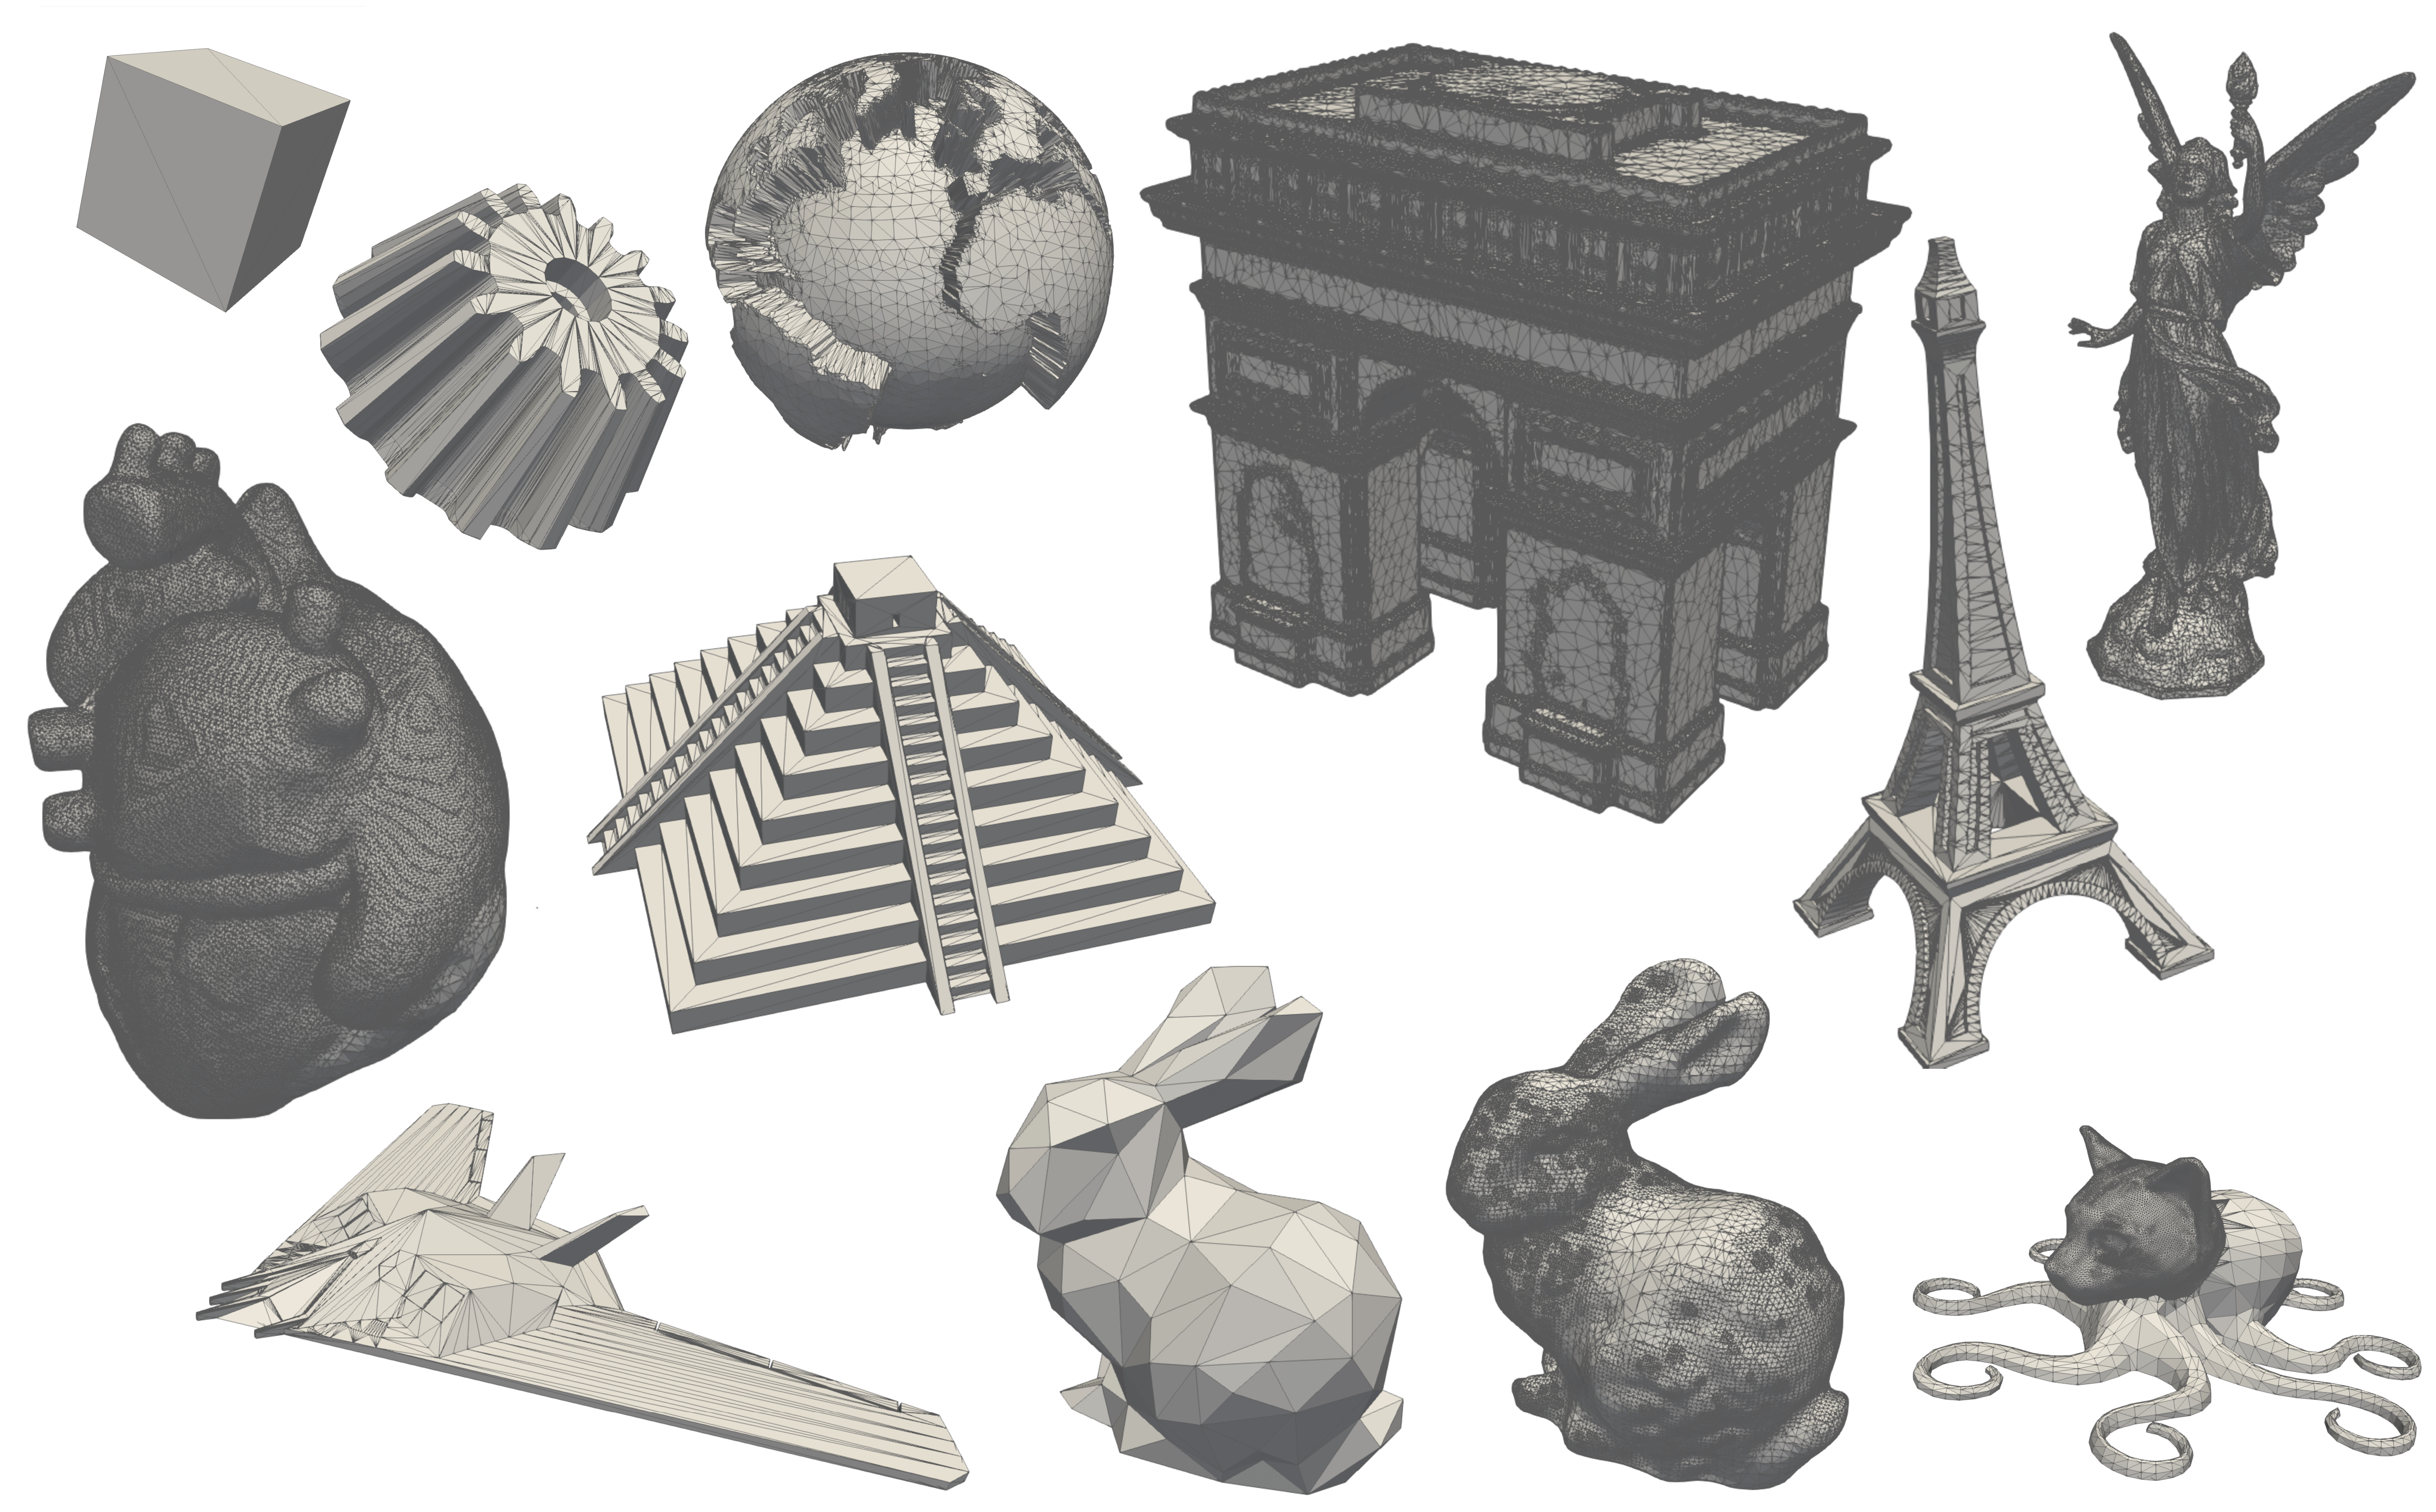
\includegraphics[width=0.95\textwidth]{matrix.pdf}
\end{frame}

\begin{frame}{1.1. Relative position - Robustness test}
  \begin{block}{Setup}
    13 STLs; 17 relative positions; 17 rotation angles;  $\{\Delta x, \theta\} = 10^{-17:-1}$
  \end{block}
  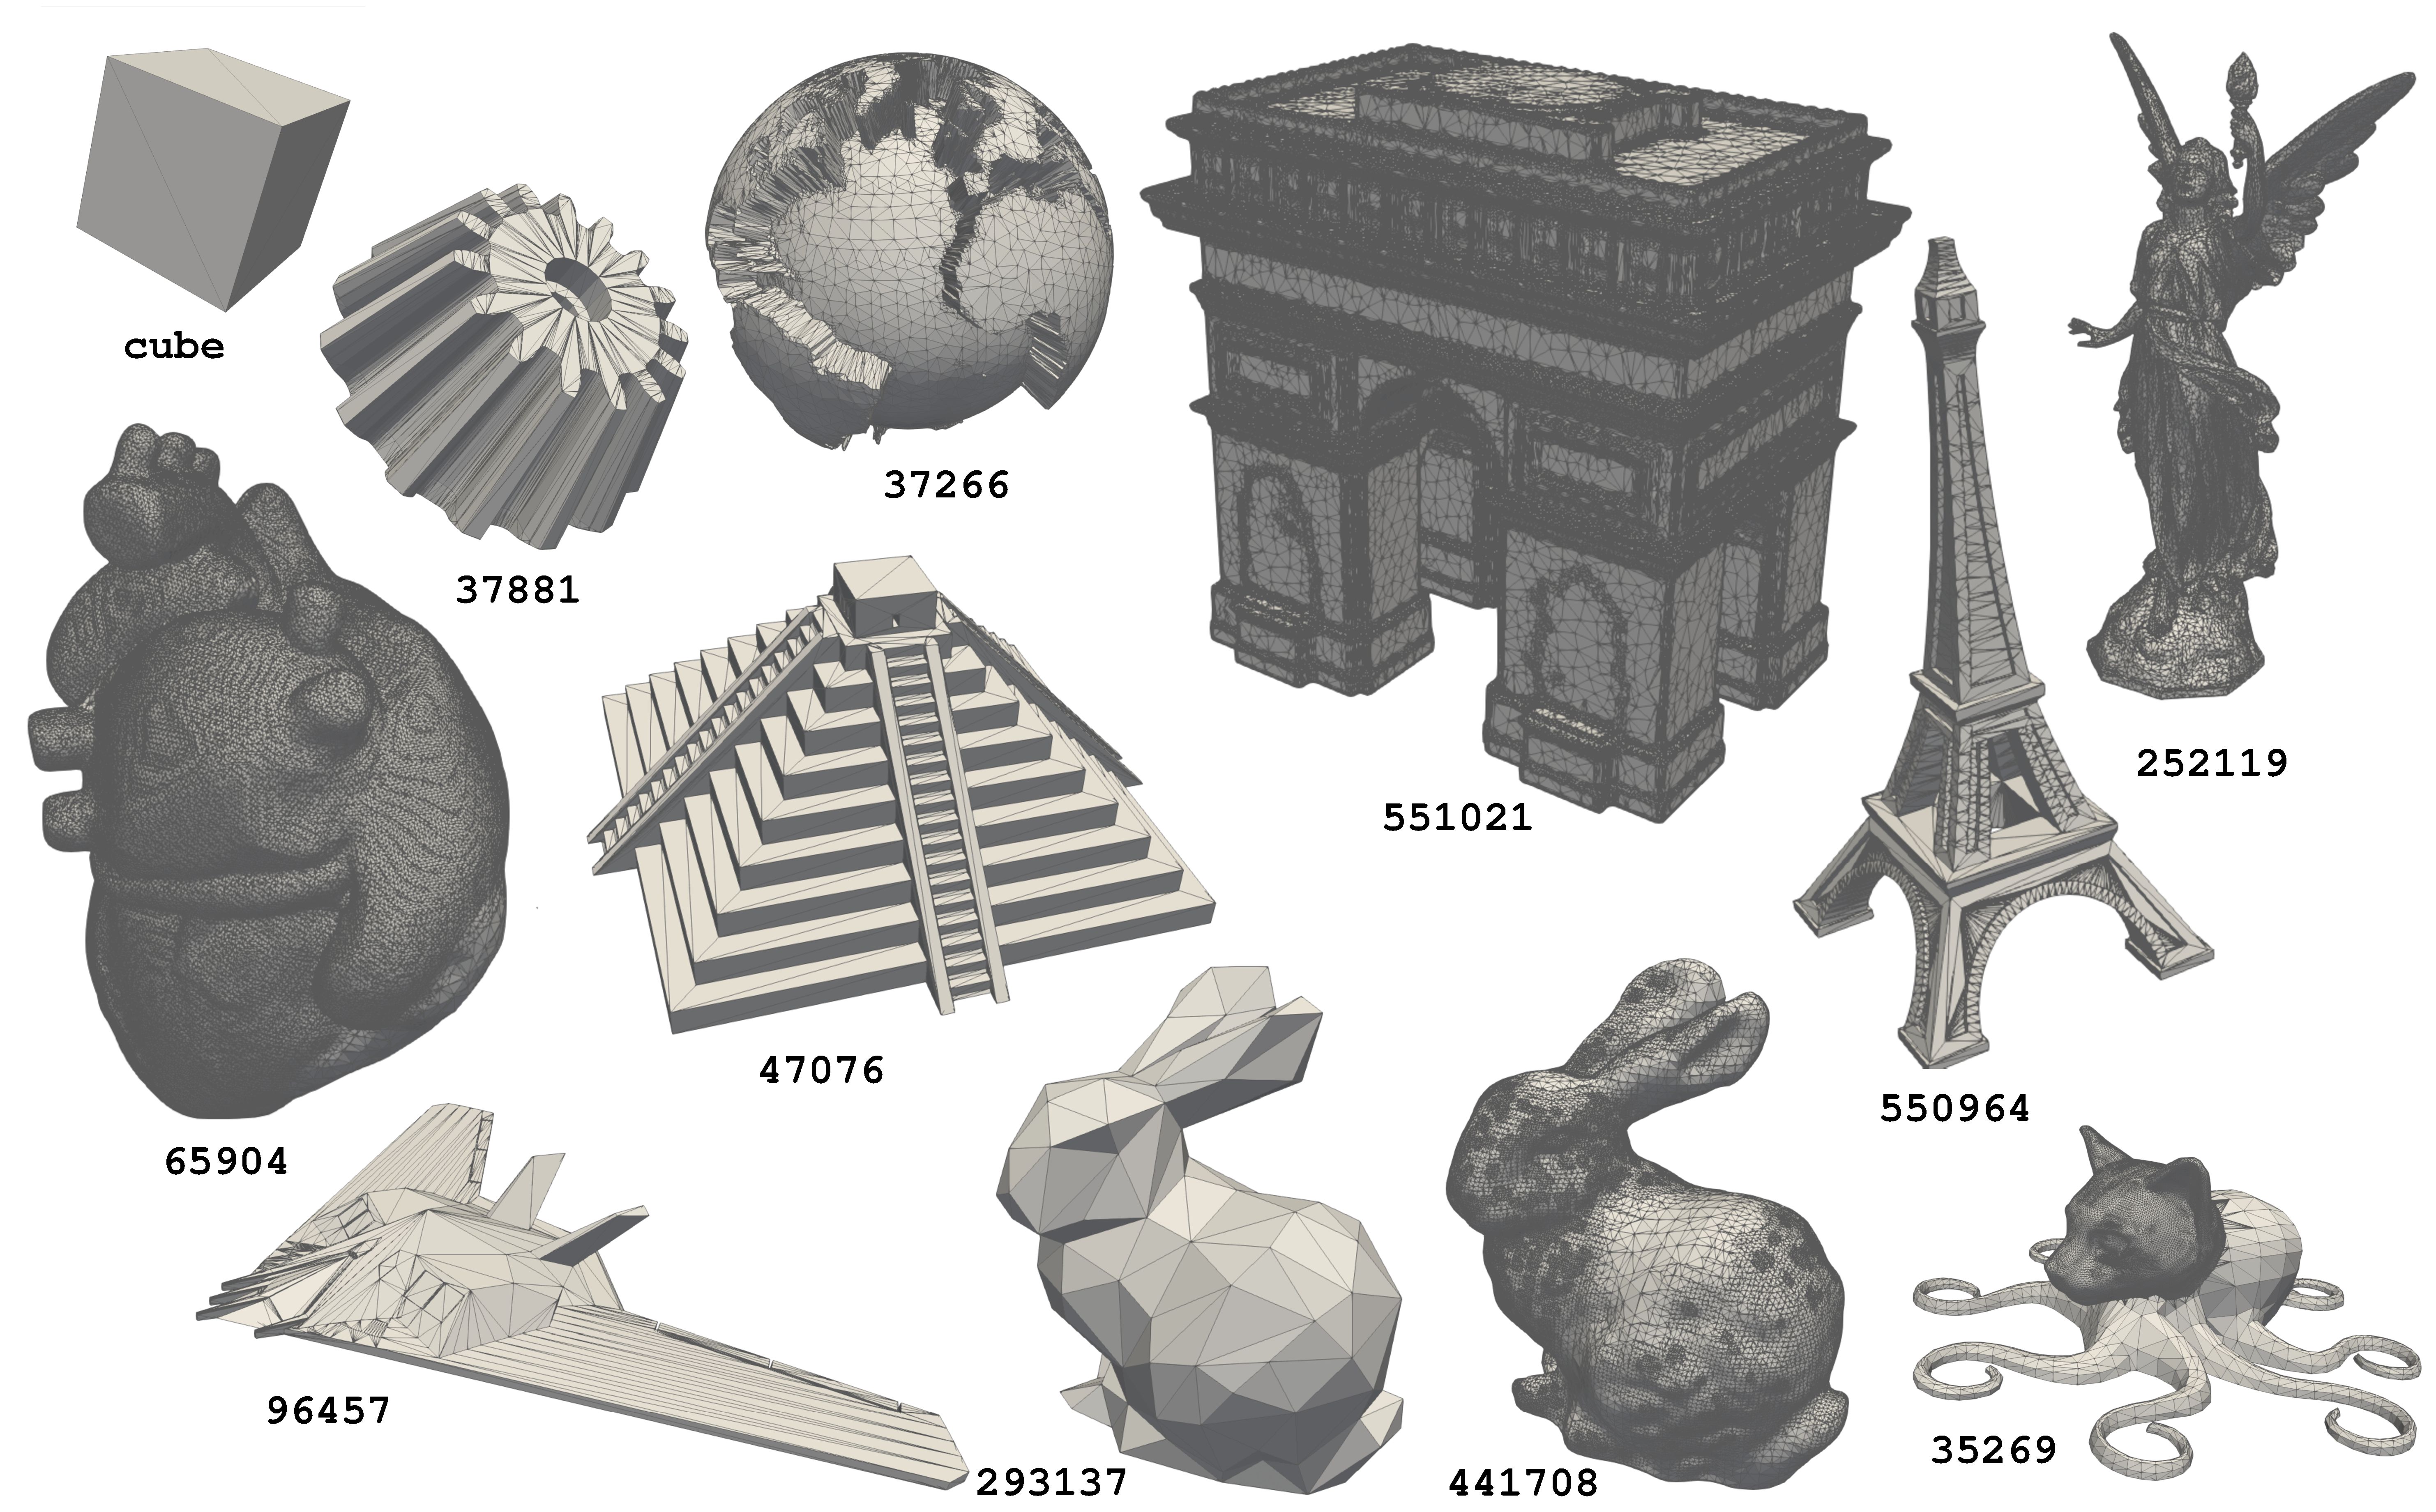
\includegraphics[width=0.95\textwidth]{matrix_ids.pdf}
\end{frame}
% thingiverse.com/download:$id
% thingiverse.com/thing:$id (wine glass)
% cube: https://people.sc.fsu.edu/~jburkardt/data/stlb/stlb.html

\begin{frame}{1.1. Relative position - Robustness test}

  \begin{block}{Domain volume variation}
  \begin{itemize}
    \item
      Maximum volume variation $< 10^{-14}$
  \end{itemize}
  \end{block}

  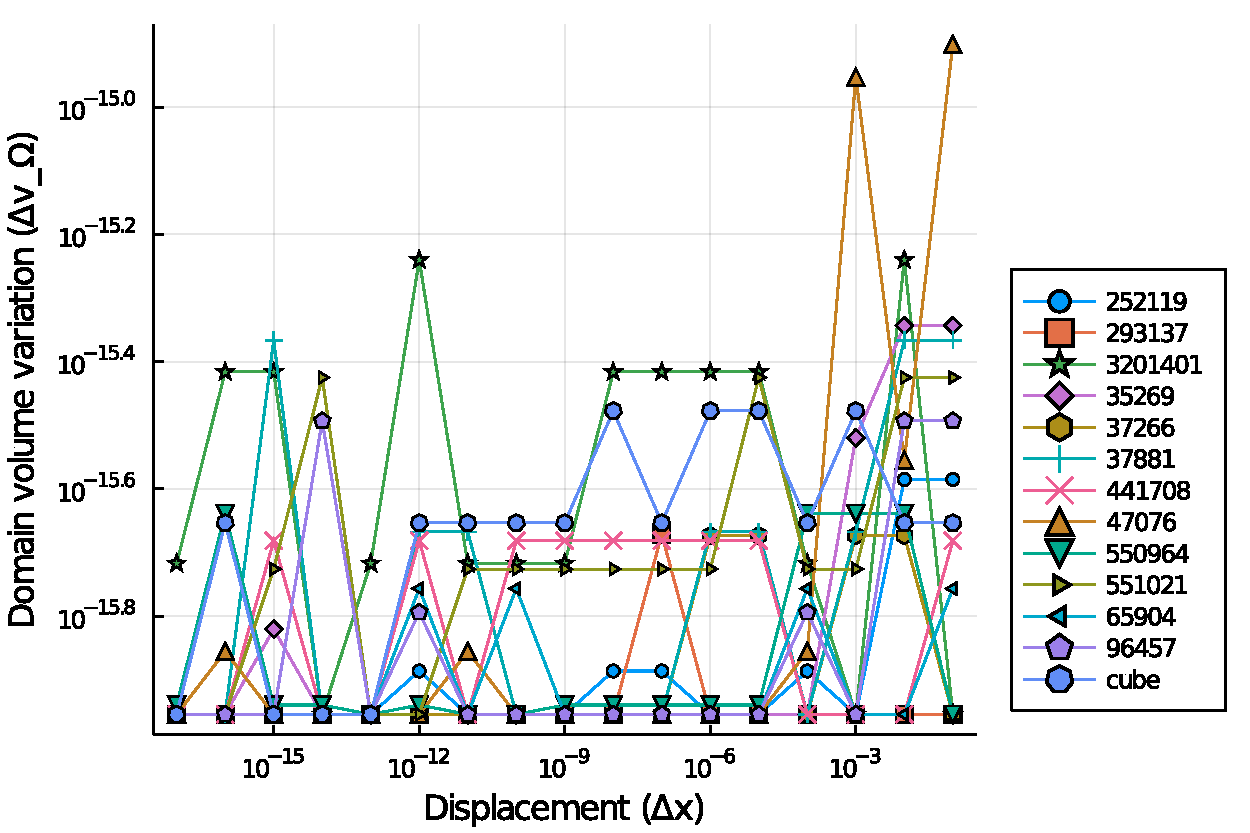
\includegraphics[width=0.49\textwidth]{../analysis/plots/x_displacement_y_domain_volume}
  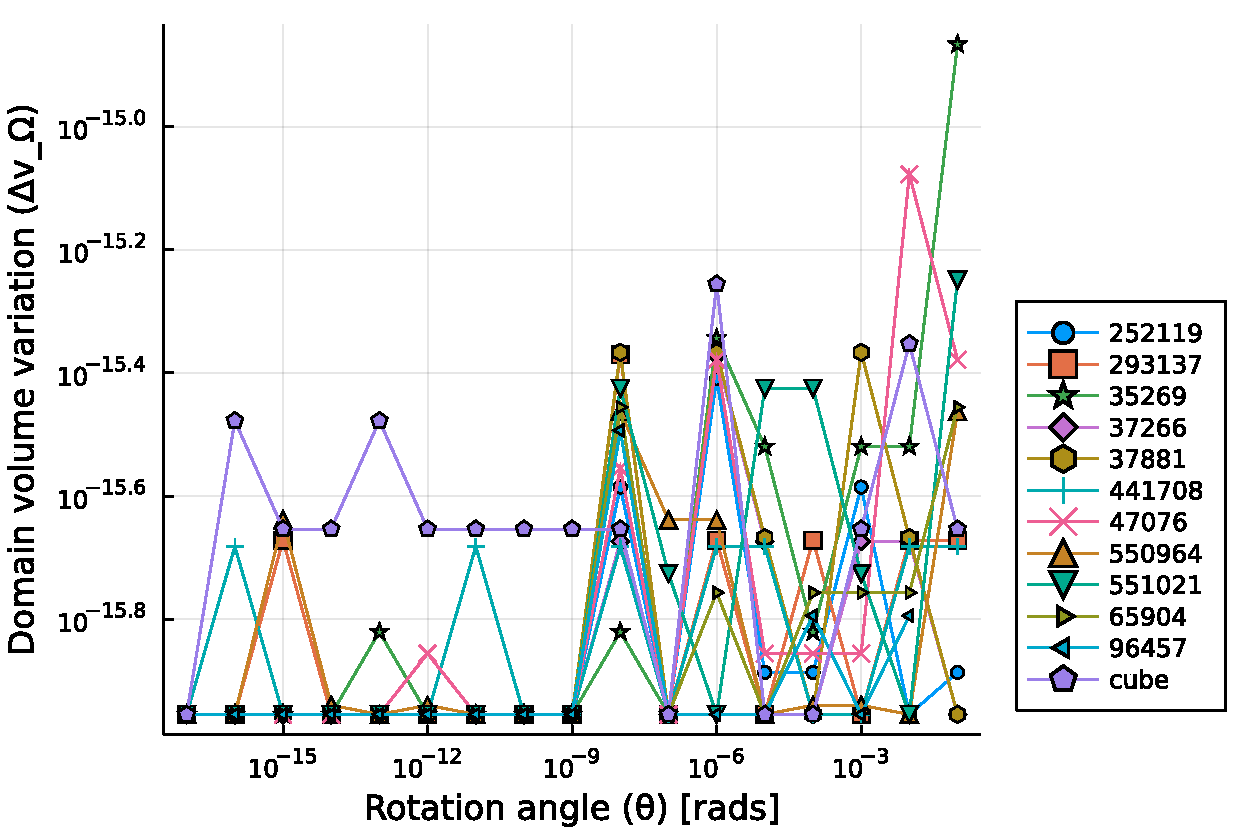
\includegraphics[width=0.49\textwidth]{../analysis/plots/x_rotation_y_domain_volume}
\end{frame}

\begin{frame}{1.1. Relative position - Robustness test}

  \begin{block}{Domain volume variation}
  \begin{itemize}
    \item
      Maximum volume variation $< 10^{-11}$
    \item
      Rotations introduce more rounding errors at planes
  \end{itemize}
  \end{block}

  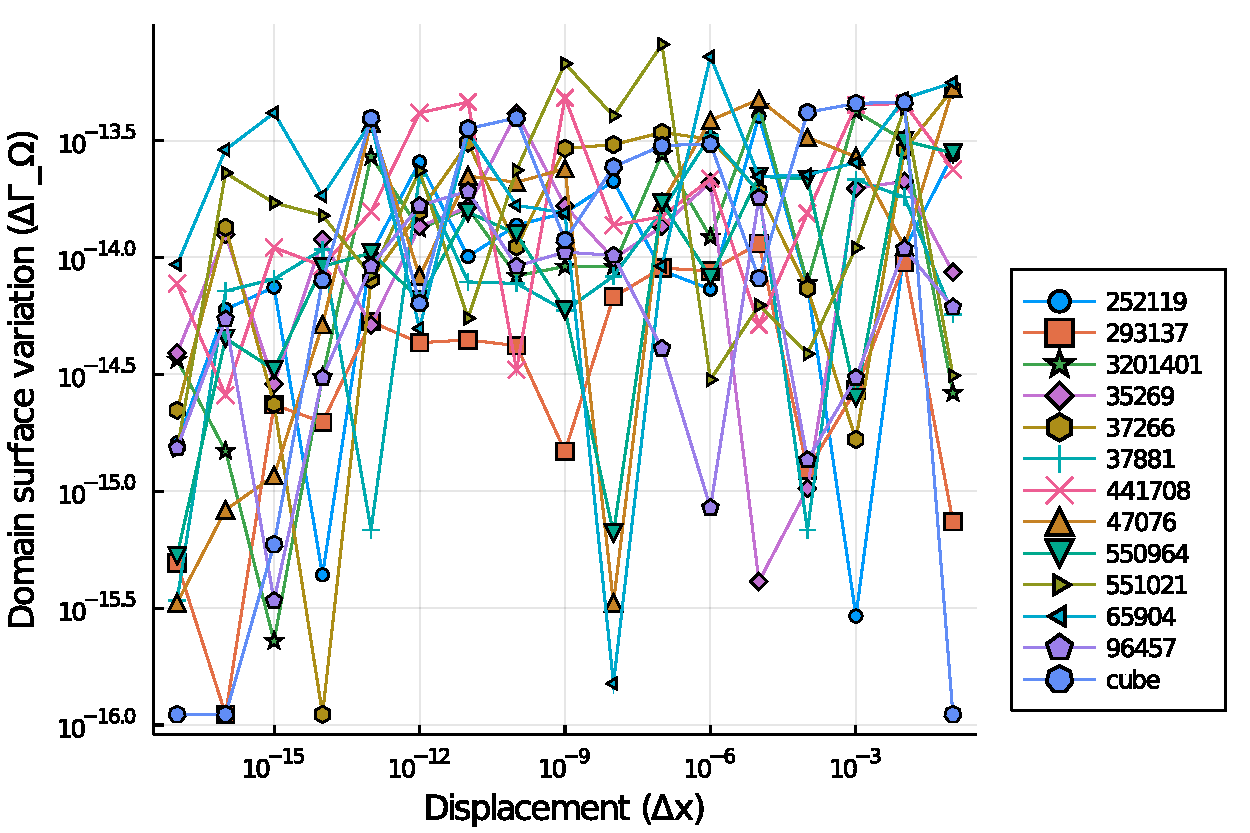
\includegraphics[width=0.49\textwidth]{../analysis/plots/x_displacement_y_domain_surface}
  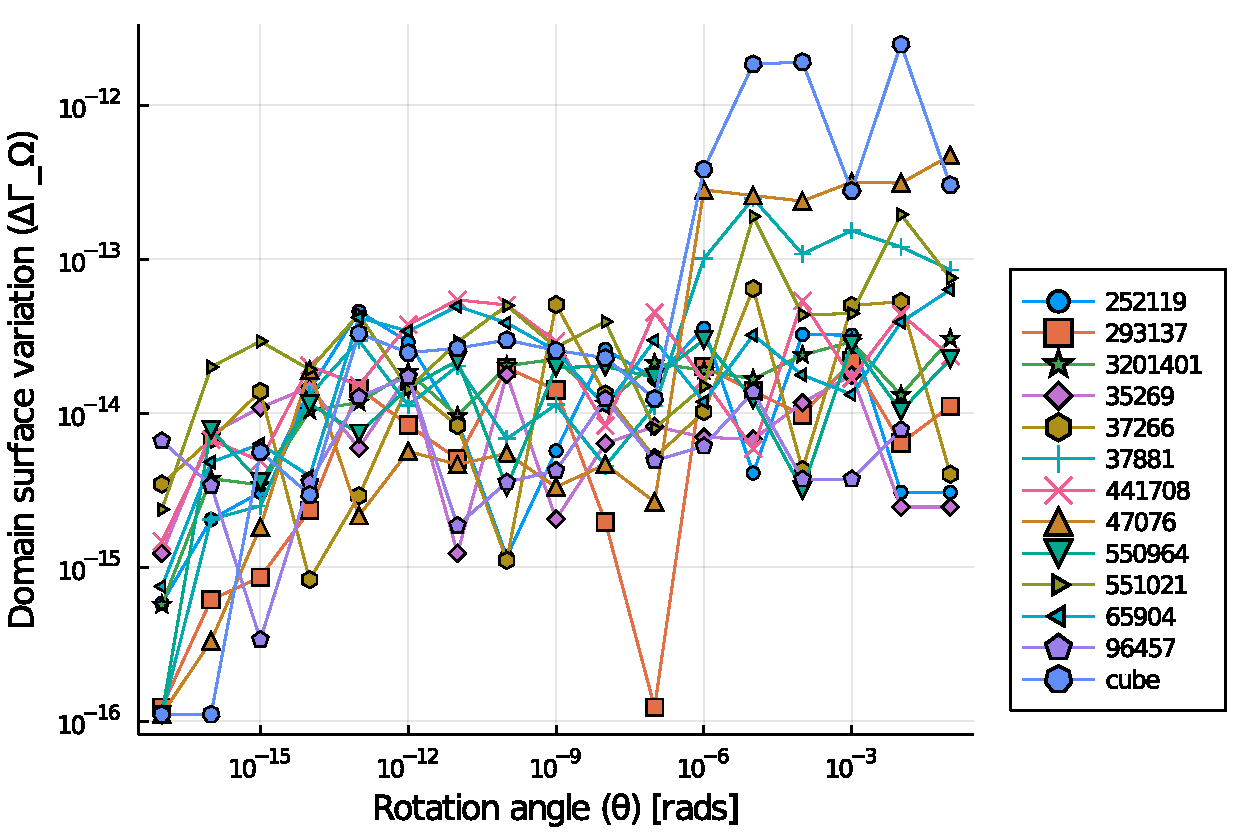
\includegraphics[width=0.49\textwidth]{../analysis/plots/x_rotation_y_domain_surface}
\end{frame}


\begin{frame}{2.1. $h$-refinement - Robustness test}
  \begin{block}{Setup}
    \begin{itemize}
      \item
        13 geometries from 1.1.
      \item
        6 refinement sizes: $N_{max} = 14 \cdot 2^{0:5}$
    \end{itemize}
  \end{block}

  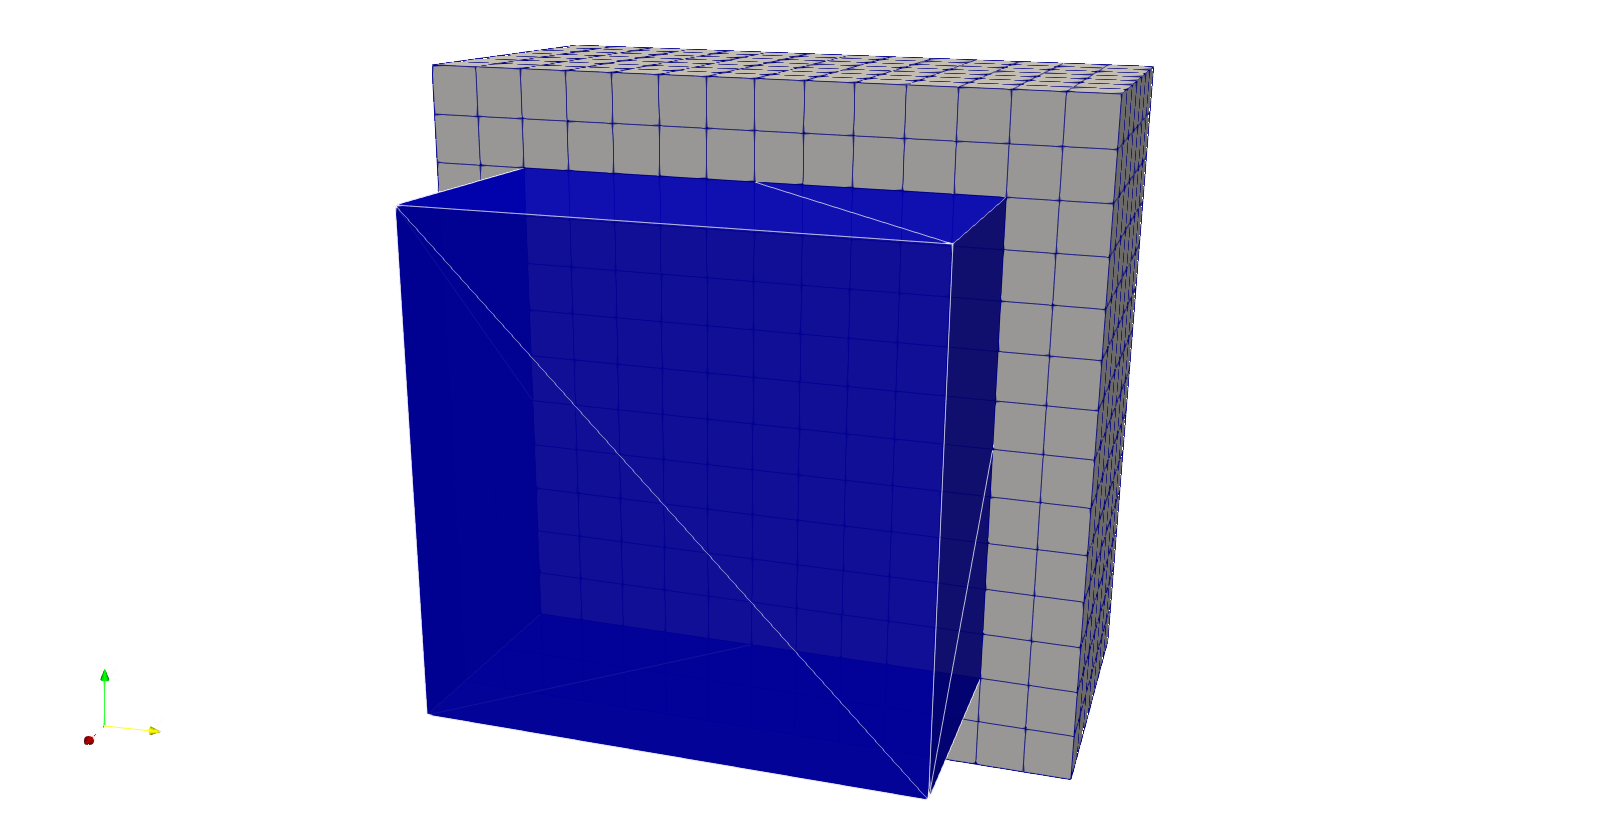
\includegraphics[width=0.7\textwidth]{cube_bb}

  \textbf{NOTE 1:} The $N_{max}$ is multiple of 14 to force the STL faces and background cell faces to be aligned, thus stress more the algorithm. As the background mesh is expanded 0.2 in each direction of the STL's bounding box.
\end{frame}

\begin{frame}{2.1. $h$-refinement - Robustness test}
  \begin{block}{Setup}
    \begin{itemize}
      \item
        13 geometries from 1.1.
      \item
        6 refinement sizes: $N_{max} = 14 \cdot 2^{0:5}$
    \end{itemize}
  \end{block}

  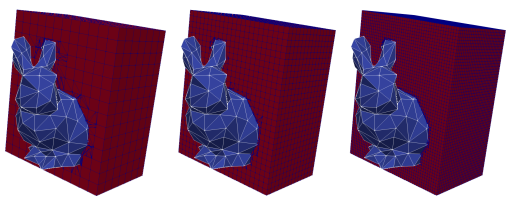
\includegraphics[width=0.95\textwidth]{h_low_bunny}

 \textbf{NOTE 2:} In order to keep the background cell aspect ratio, $N_{max}$ is the number of divisions on the largest side of the bounding box.
\end{frame}


\begin{frame}{2.1. $h$-refinement - Robustness test}

  \begin{block}{$h$-refinement}
  \begin{itemize}
    \item
      Surface variation increases with $1/h$ ($\Delta \Gamma < 10^{-11}$)
    \item
      Volume is constant at refinement ($\Delta V < 10^{-14}$)
  \end{itemize}
  \end{block}

  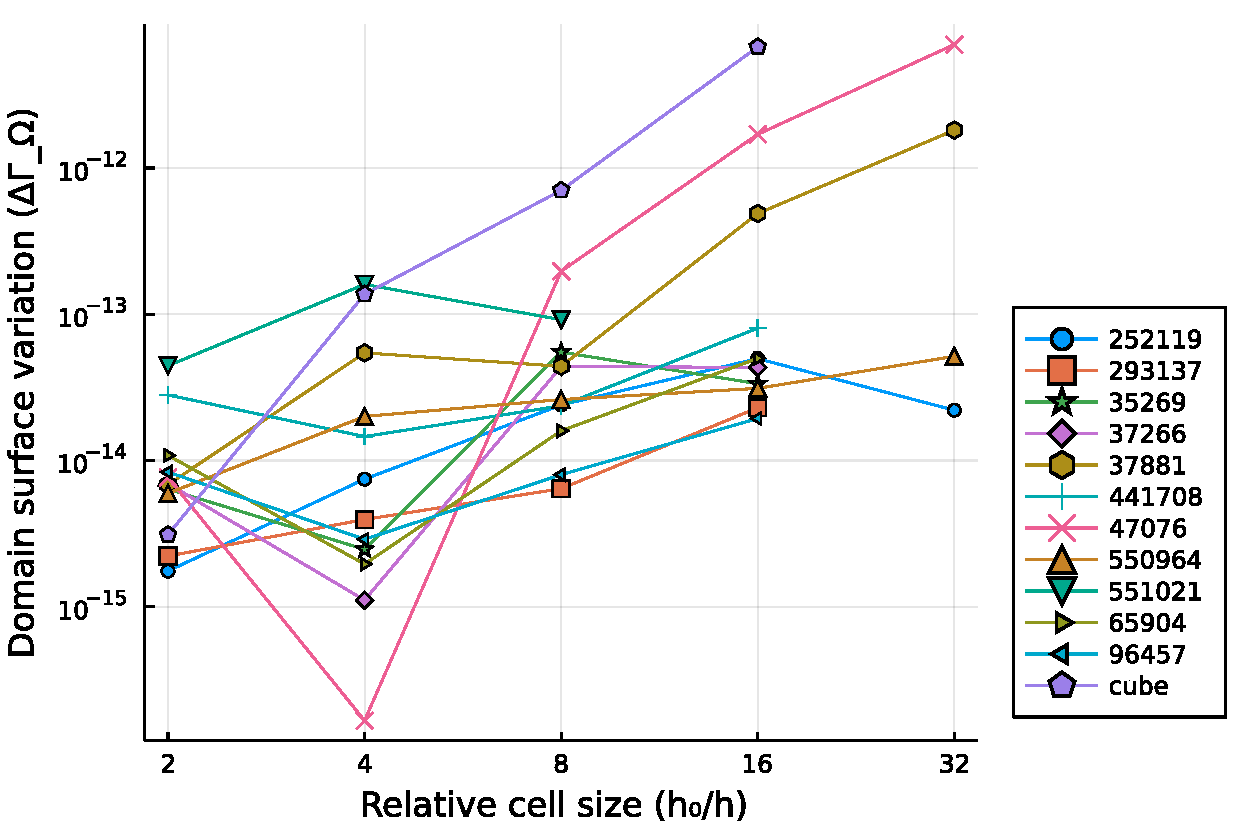
\includegraphics[width=0.49\textwidth]{../analysis/plots/x_nmax_y_domain_surface}
  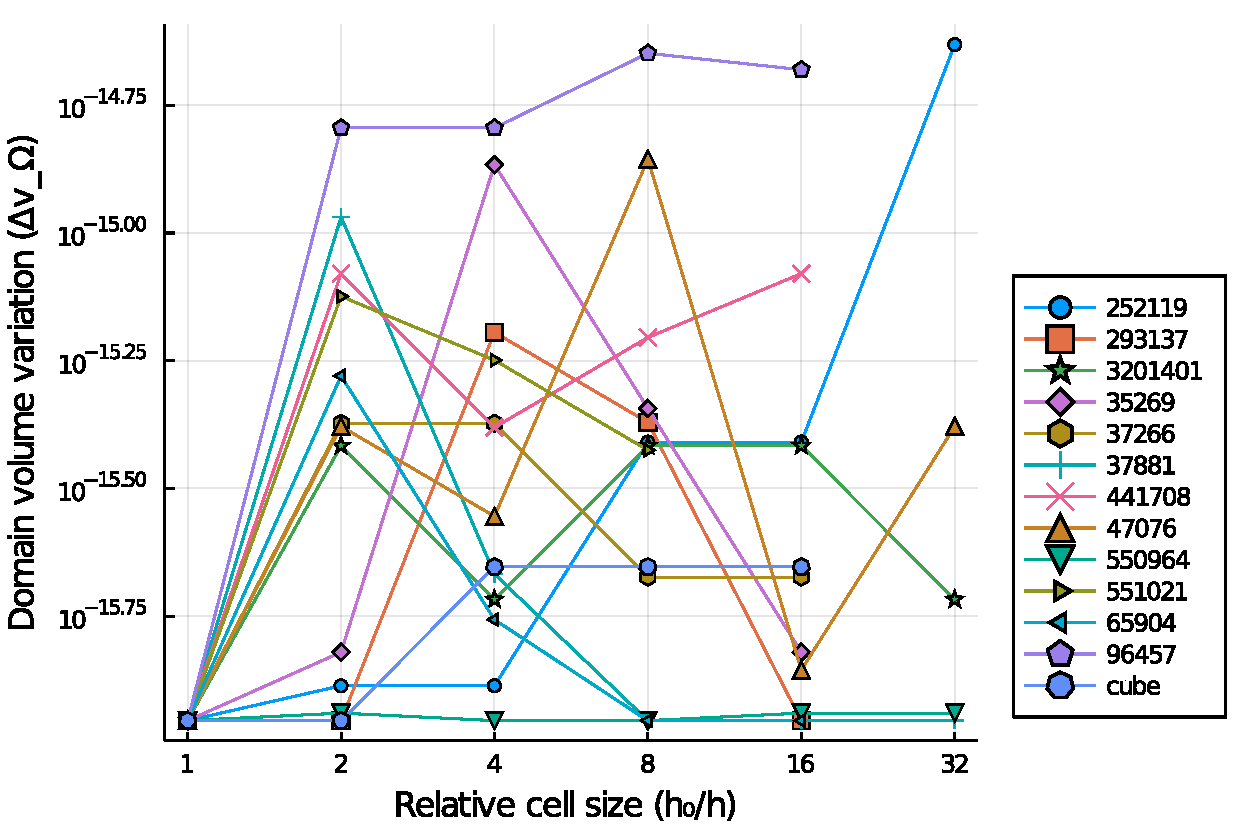
\includegraphics[width=0.49\textwidth]{../analysis/plots/x_nmax_y_domain_volume}
\end{frame}

\begin{frame}{Robustness matrix}

  \begin{block}{CPU time with $h$-refinement}
  \begin{itemize}
    \item
      Not precise measure (single runs)
    \item
      Tend to be linear after first complexity reduction
  \end{itemize}
  \end{block}

  \centering
  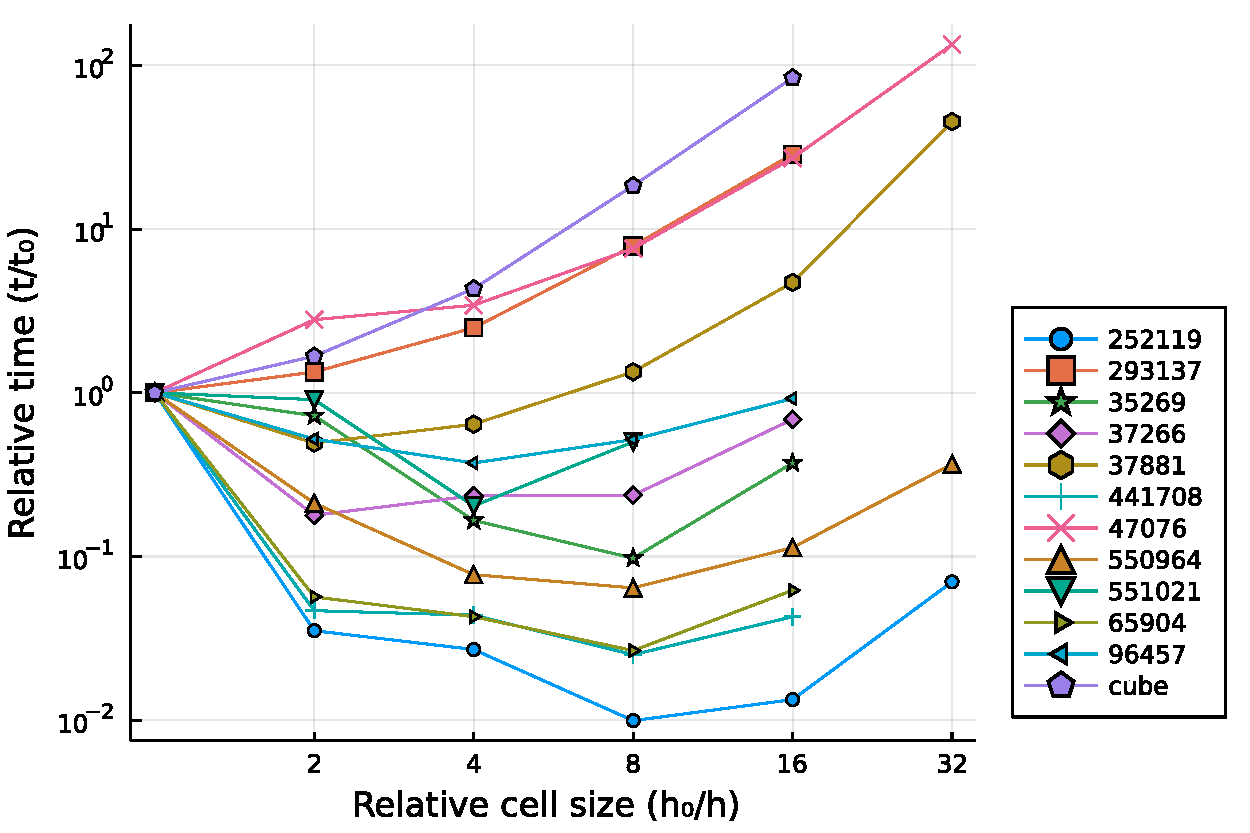
\includegraphics[width=0.60\textwidth]{../analysis/plots/x_nmax_y_time}

\end{frame}


\begin{frame}{Large geometry dataset}
  \begin{block}{Setup}
    \begin{itemize}
      \item
  
        \href{https://ten-thousand-models.appspot.com/results.html?q=is+closed\%2C+is+oriented\%2C+is+manifold\%2C+is+not+degenerate\%2C+without+self-intersection\%2C+\%23df\%3D0}{\underline{5052 geometries}}
        filtered from \href{https://ten-thousand-models.appspot.com}{Thingi10k}

        
      \item
        $N_{max} = 100 $ (unique $h$-refinement criterion)
    \end{itemize}

  \end{block}


\end{frame}
\begin{frame}{Thingi 10k dataset}
  \begin{block}{Summary}
   \dirtree{%
     .1 Total = 5052  .
     .2 Not available: 312 .
     .2 Load error: 7 .
     .2 Available: 4733 .
     .3 Launched on HPC: 4072.
     .4 Success: 3986 .
     .4 Large volume error: 53 .
     .4 Not ended: 33 .
     .3 Pending: 661 .
     }

  \end{block}

  \vfill{}

  \textbf{NOTE:} As shown in next slides large volume error is due to small facets.

%  \framesubtitle{Few numbers}
%
%  Num geometries: 5052
%
%  Not available: 312 (6.2\% of total)
%
%  Load error: 7 (0.14\% of total)
%
%  Available: 5052-312-7=4733 (93.7\% of total)
%
%  \textbf{Success geometries:} 3817 (78.5\% of available, 97.4\% of launched)
%
%  Large volume error ($>$1e-14): 67 (1.8\% of success) (100\% due to small facets)
%
%  Found to be degenerated: 4
%
%  Failed: 34 (0.89\% of success)
%
%  Missing (running): 916 (19.4\% of total)
%  \vfill{}
%  \textbf{ONGOING:}
%  Try to fix problems with small facets
%  Indentify failed runs as degenerate or fix
%
%

\end{frame}


\begin{frame}{Thingi 10k dataset}

  \begin{block}{Volume error}
  \begin{itemize}
    \item
      $\epsilon_V = V_{IN} + V_{OUT} - V_{BBOX}$
    \item
      98.7\% of 4039 is below $10^{-9}$
    \item
      All STLs above $10^{-9}$ contain small facets
  \end{itemize}
  \end{block}

  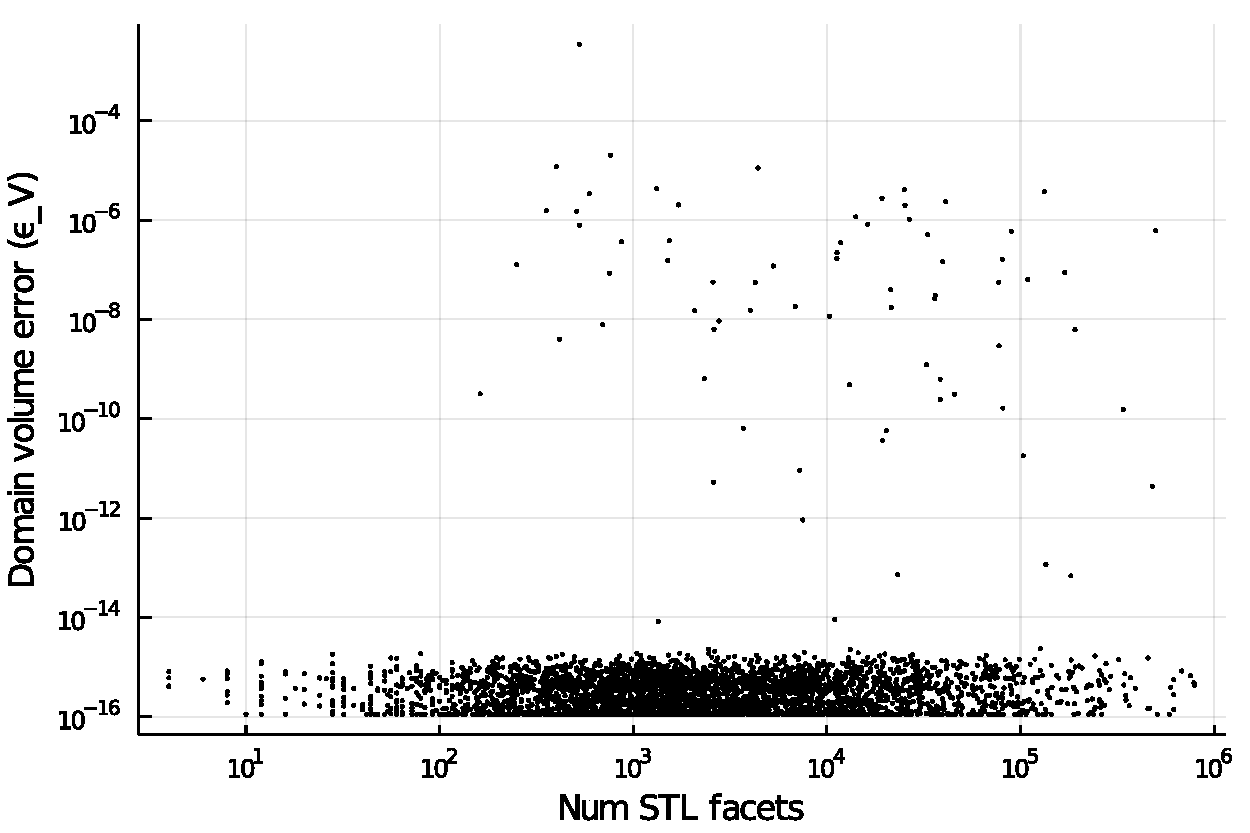
\includegraphics[width=0.49\textwidth]{../analysis/plots/num_stl_facets_volume_error}
  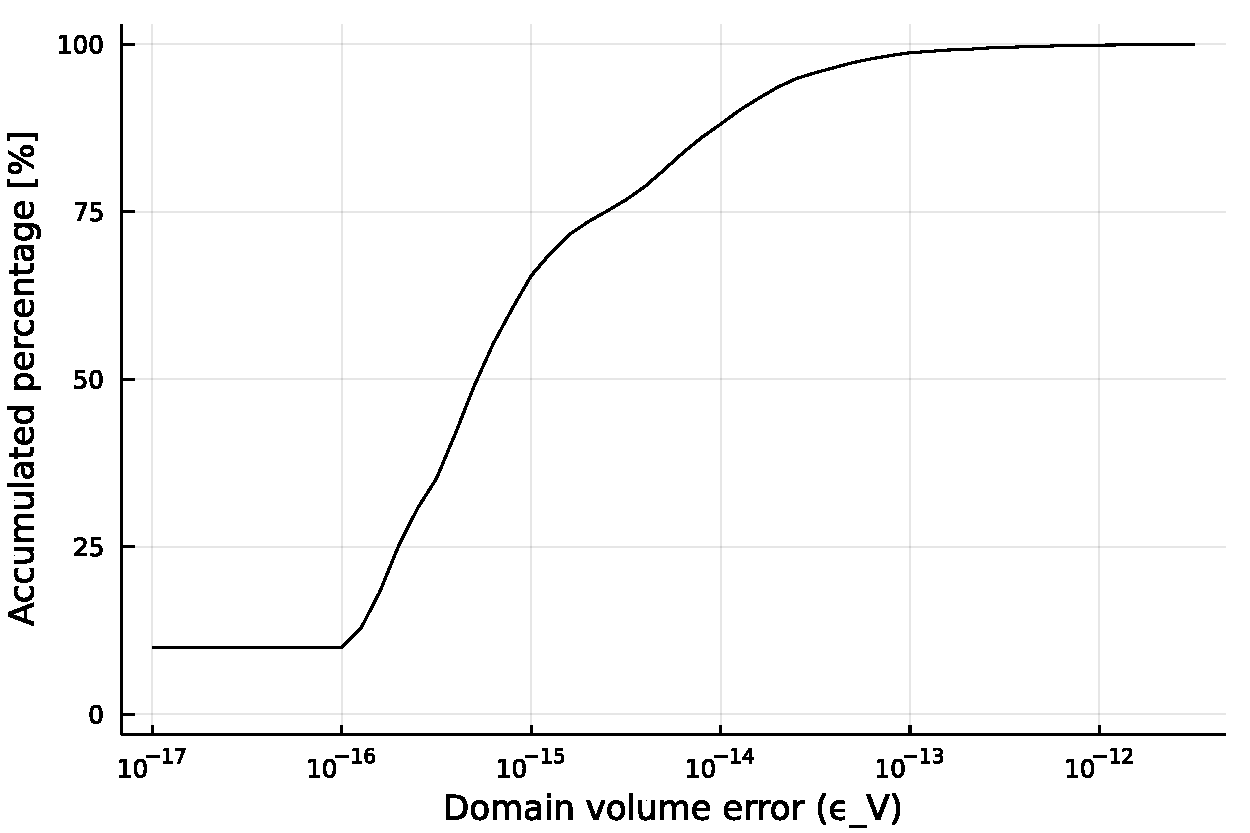
\includegraphics[width=0.49\textwidth]{../analysis/plots/histogram_volume_error}
\end{frame}

\begin{frame}{Thingi 10k dataset}

  \begin{block}{Volume error}
  \begin{itemize}
    \item
      $\epsilon_V = V_{IN} + V_{OUT} - V_{BBOX}$
    \item
      98.7\% of 4039 is below $10^{-9}$
    \item
      All STLs above $10^{-9}$ contain small facets
  \end{itemize}
  \end{block}

  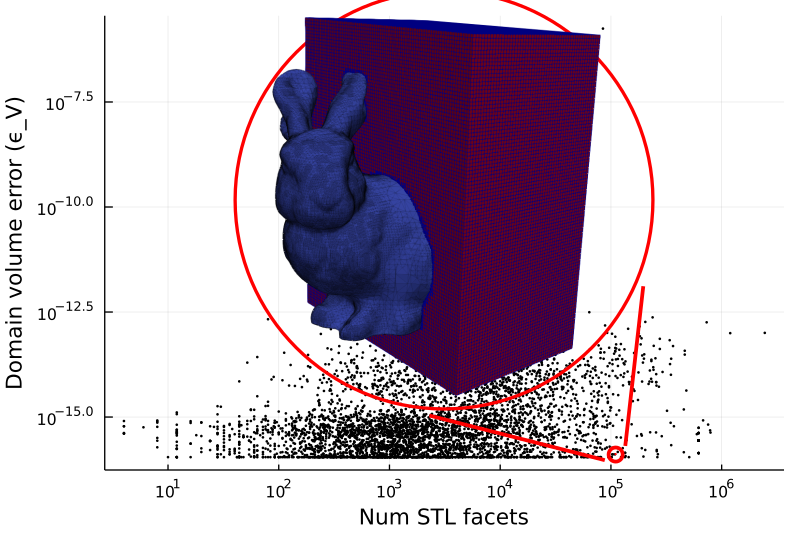
\includegraphics[width=0.49\textwidth]{num_stl_facets_volume_error_bunny}
  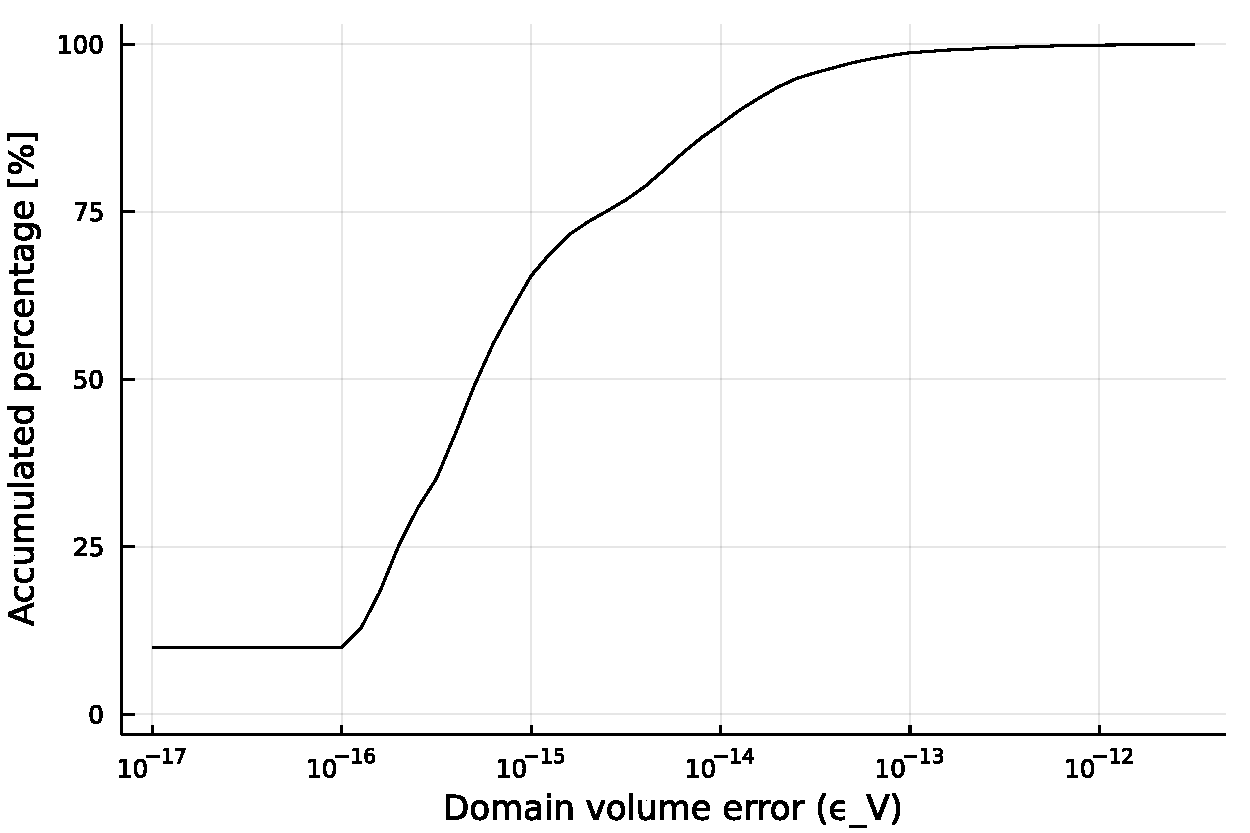
\includegraphics[width=0.49\textwidth]{../analysis/plots/histogram_volume_error}
\end{frame}

\begin{frame}{Thingi 10k dataset}

  \begin{block}{Volume error}
  \begin{itemize}
    \item
      $\epsilon_V = V_{IN} + V_{OUT} - V_{BBOX}$
    \item
      98.7\% of 4039 is below $10^{-9}$
    \item
      All STLs above $10^{-9}$ contain small facets
  \end{itemize}
  \end{block}

  \includegraphics[width=0.49\textwidth]{num_stl_facets_volume_error_509317}
  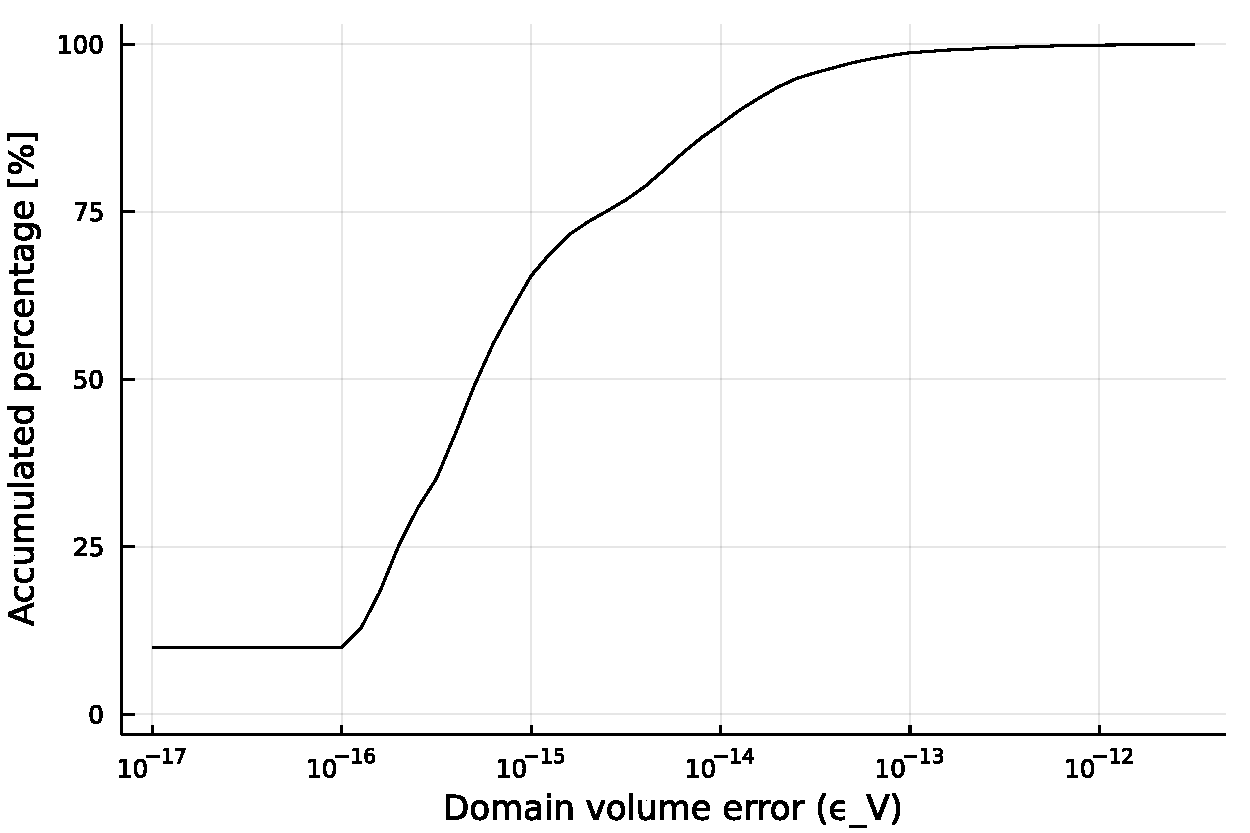
\includegraphics[width=0.49\textwidth]{../analysis/plots/histogram_volume_error}
\end{frame}

\begin{frame}{Thingi 10k dataset}

  \begin{block}{Volume error [filtering STLs with small facets]}
  \begin{itemize}
    \item
      $\epsilon_V = V_{IN} + V_{OUT} - V_{BBOX}$
    \item
      100\% is below $10^{-14}$
   % \item
   %   All STLs above $10^{-9}$ contain small facets
  \end{itemize}
  \end{block}

  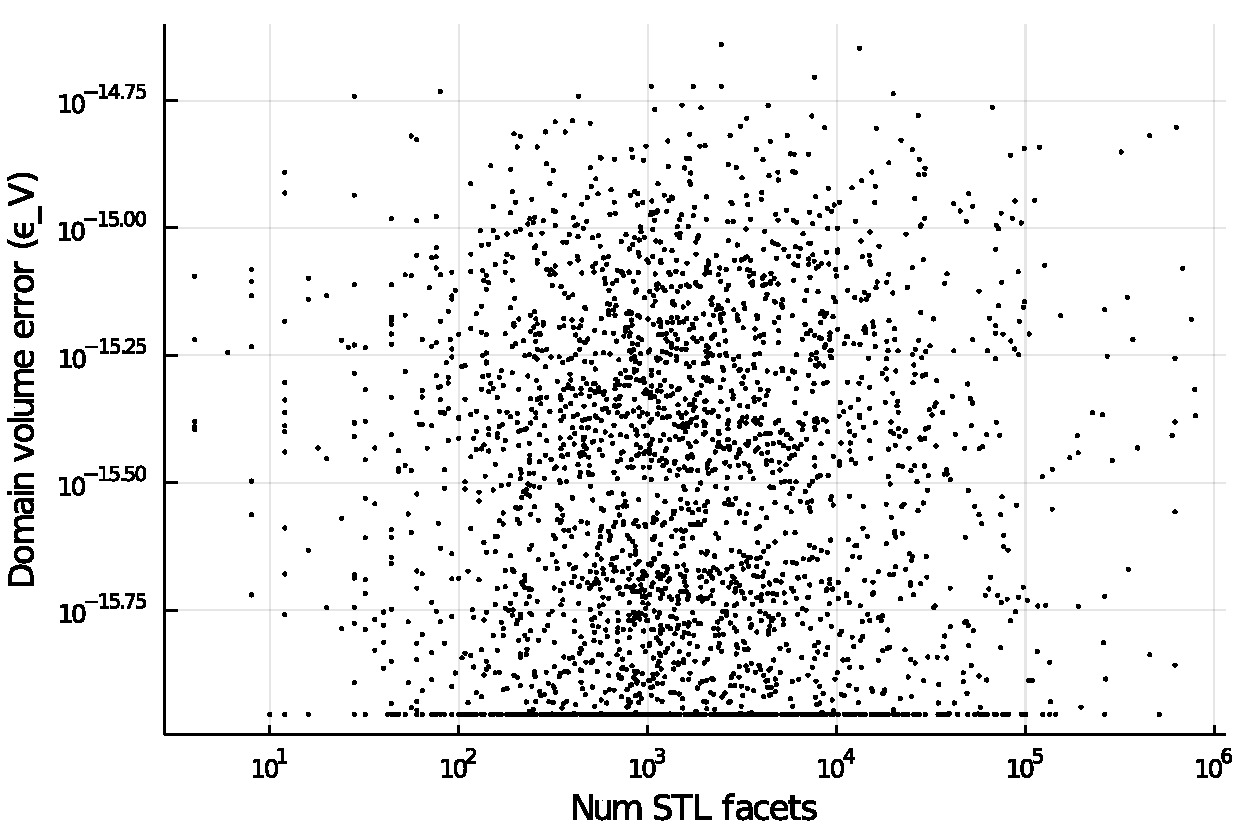
\includegraphics[width=0.49\textwidth]{../analysis/plots/filter_num_stl_facets_volume_error}
  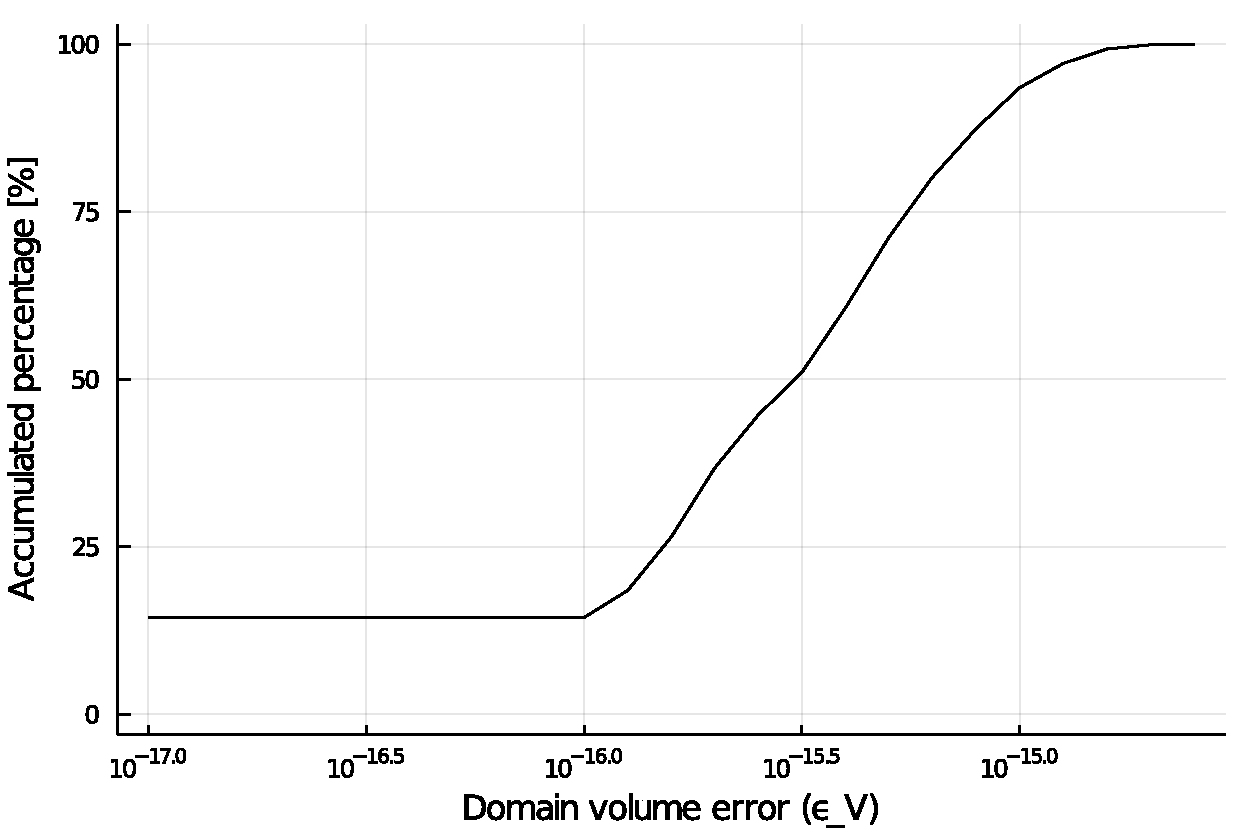
\includegraphics[width=0.49\textwidth]{../analysis/plots/filter_histogram_volume_error}
\end{frame}

\begin{frame}{Thingi 10k dataset}

  \begin{block}{Surface error}
  \begin{itemize}
    \item
      $\epsilon_\Gamma = \Gamma - V_{STL}$
    \item
      99.0\% of 4039 is below $10^{-9}$
    \item
      (almost) All STLs above $10^{-9}$ contain small facets
  \end{itemize}
  \end{block}

  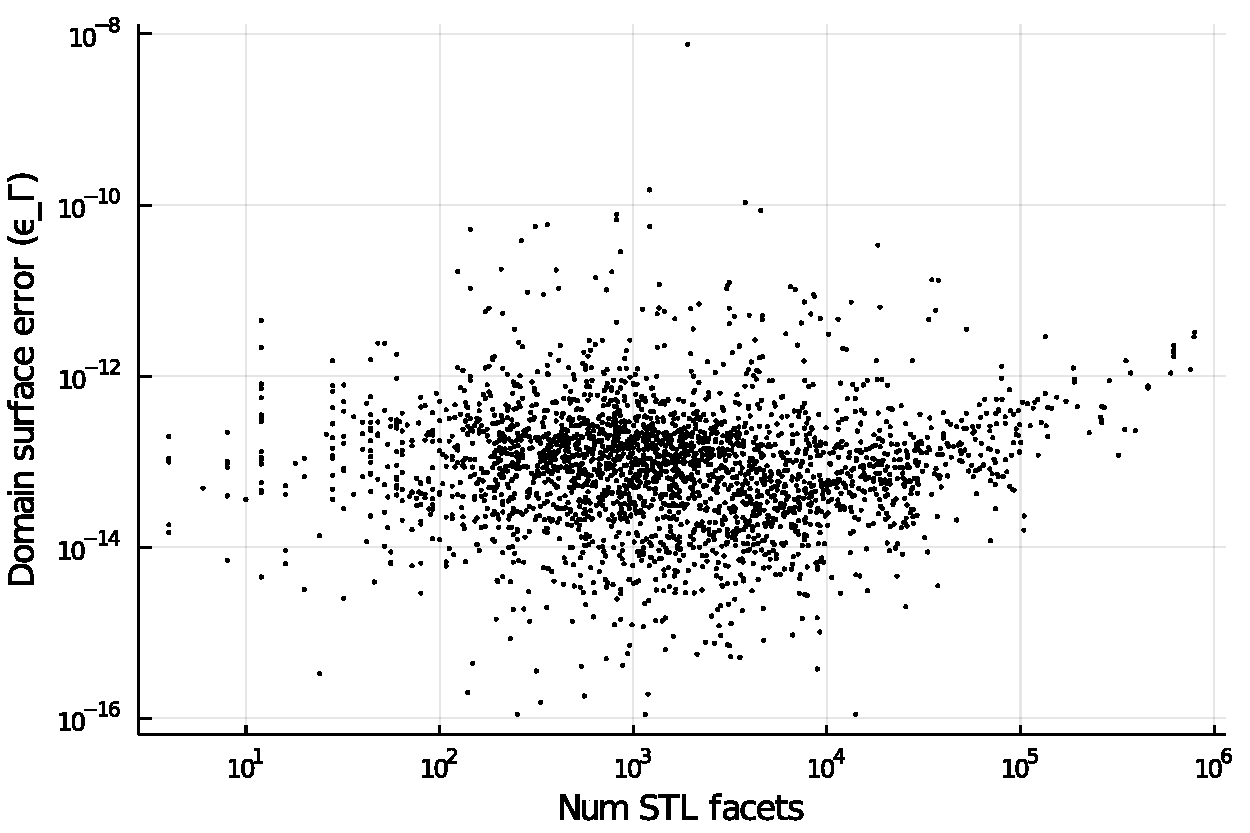
\includegraphics[width=0.49\textwidth]{../analysis/plots/num_stl_facets_surface_error}
  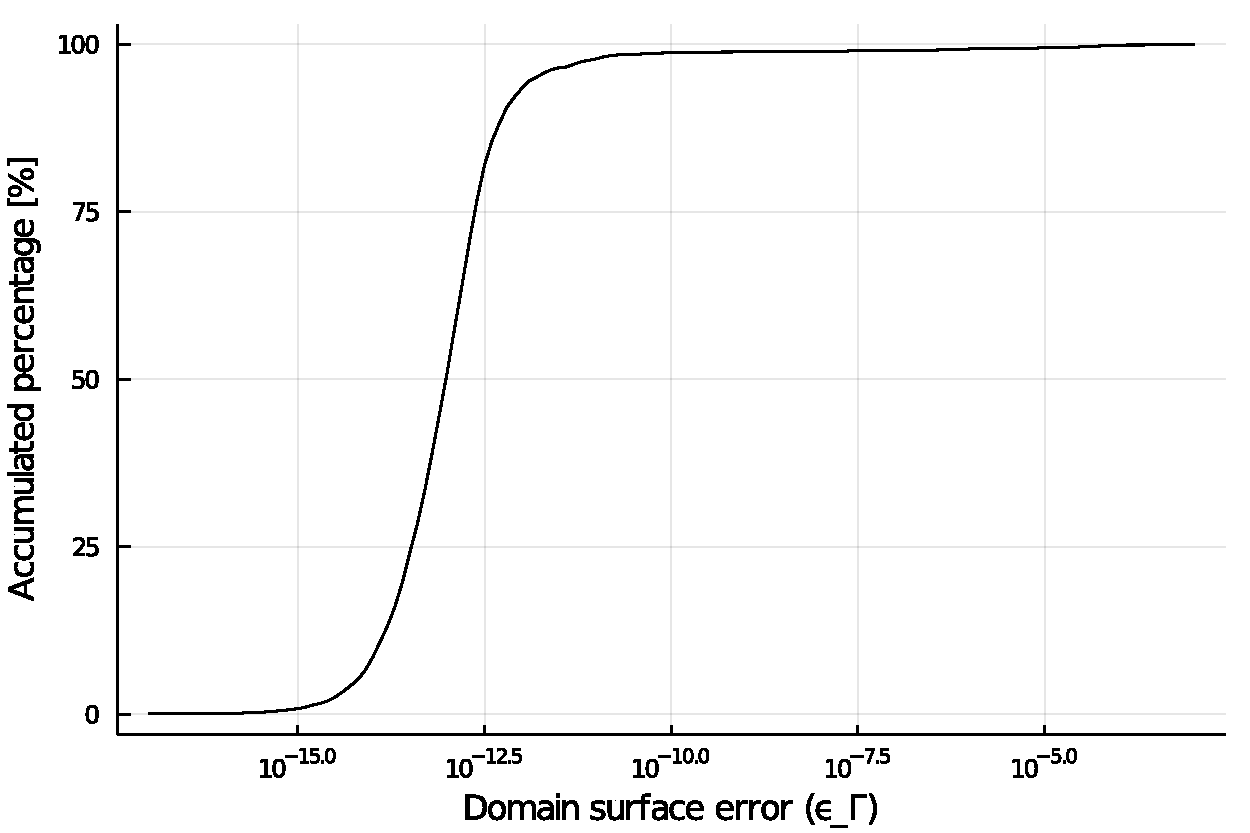
\includegraphics[width=0.49\textwidth]{../analysis/plots/histogram_surface_error}
\end{frame}

\begin{frame}{Thingi 10k dataset}

  \begin{block}{Surface error [filtering STLs with small facets]}
  \begin{itemize}
    \item
      $\epsilon_\Gamma = \Gamma - V_{STL}$
    \item
      99.9\% is below $10^{-9}$
    \item
      One outlier can be moved by increasing the tolerance
  \end{itemize}
  \end{block}

  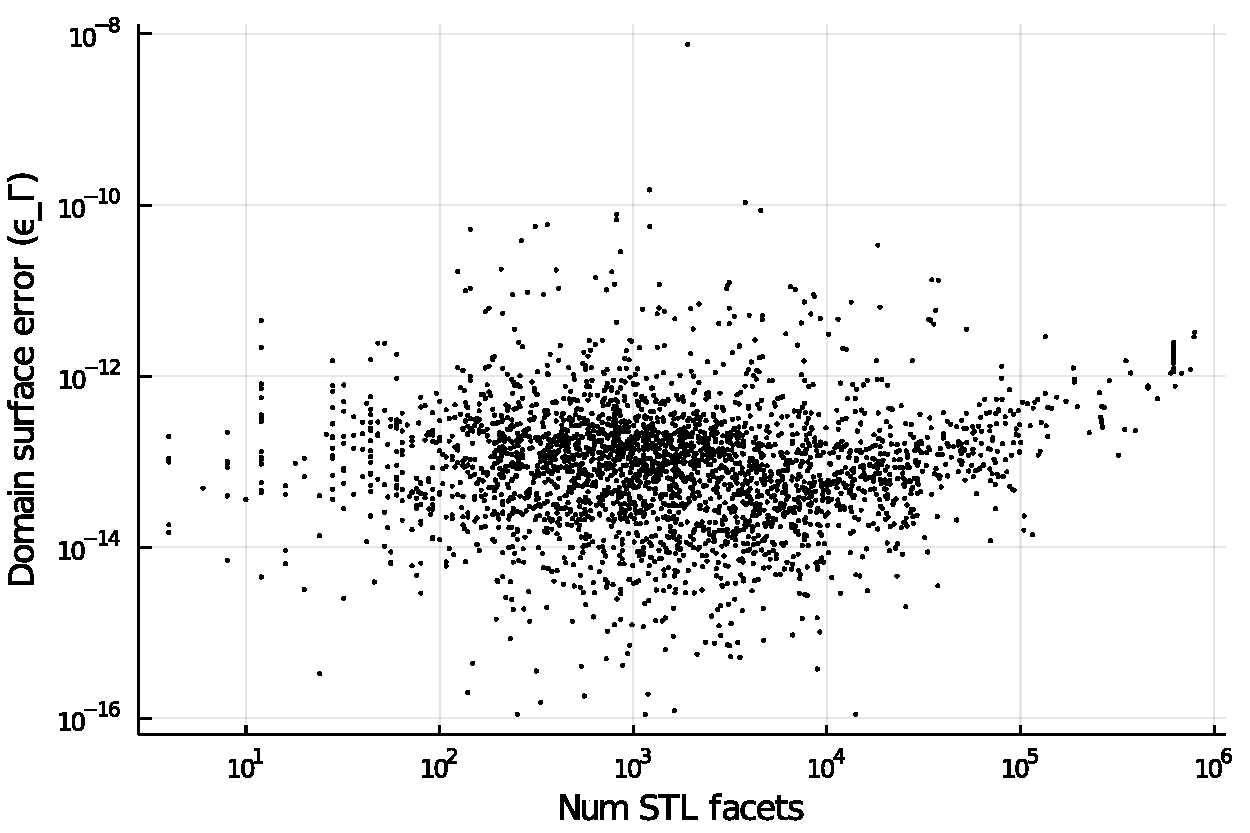
\includegraphics[width=0.49\textwidth]{../analysis/plots/filter_num_stl_facets_surface_error}
  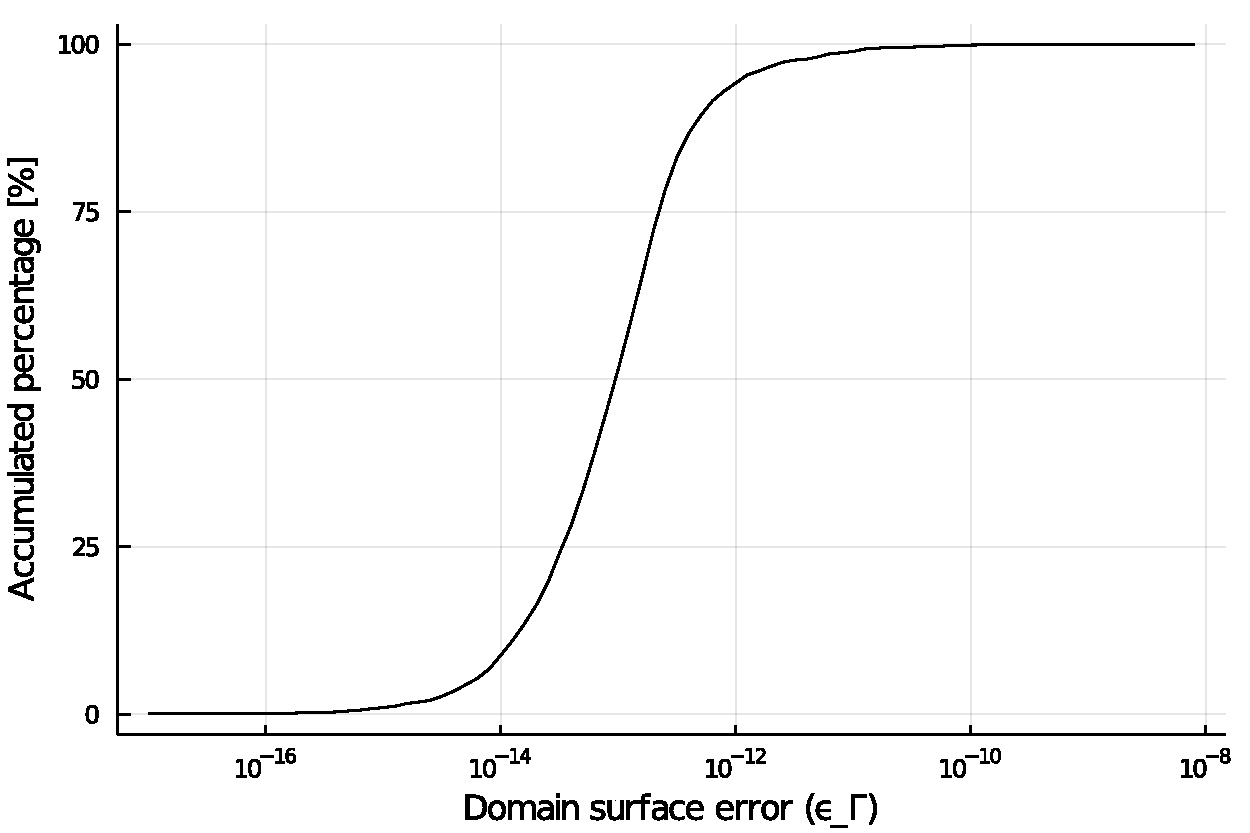
\includegraphics[width=0.49\textwidth]{../analysis/plots/filter_histogram_surface_error}
\end{frame}

\begin{frame}{Thingi 10k dataset}

  \begin{block}{Surface error [filtering STLs with small facets]}
  \begin{itemize}
    \item
      $\epsilon_\Gamma = \Gamma - V_{STL}$
    \item
      99.9\% is below $10^{-9}$
    \item
      One outlier can be moved by increasing the tolerance
  \end{itemize}
  \end{block}

  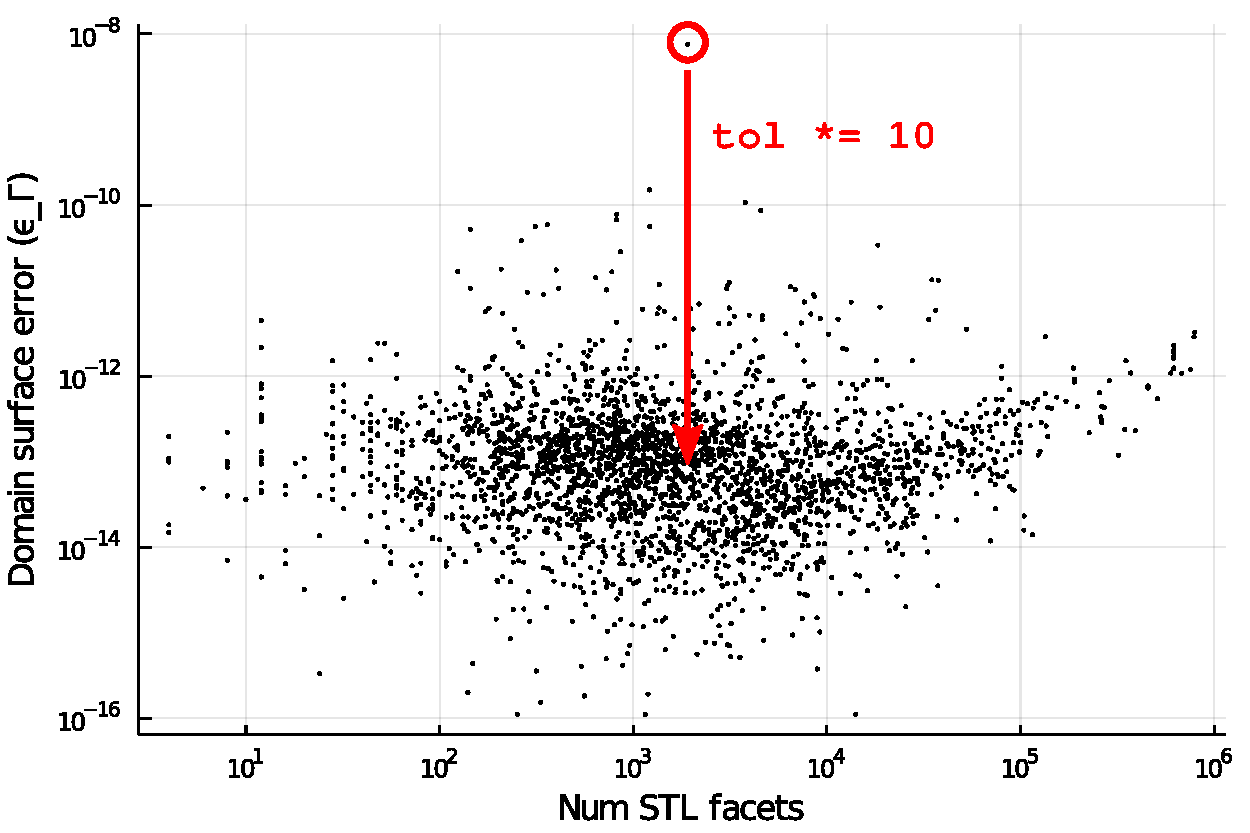
\includegraphics[width=0.49\textwidth]{moving_filter_num_stl_facets_surface_error}
  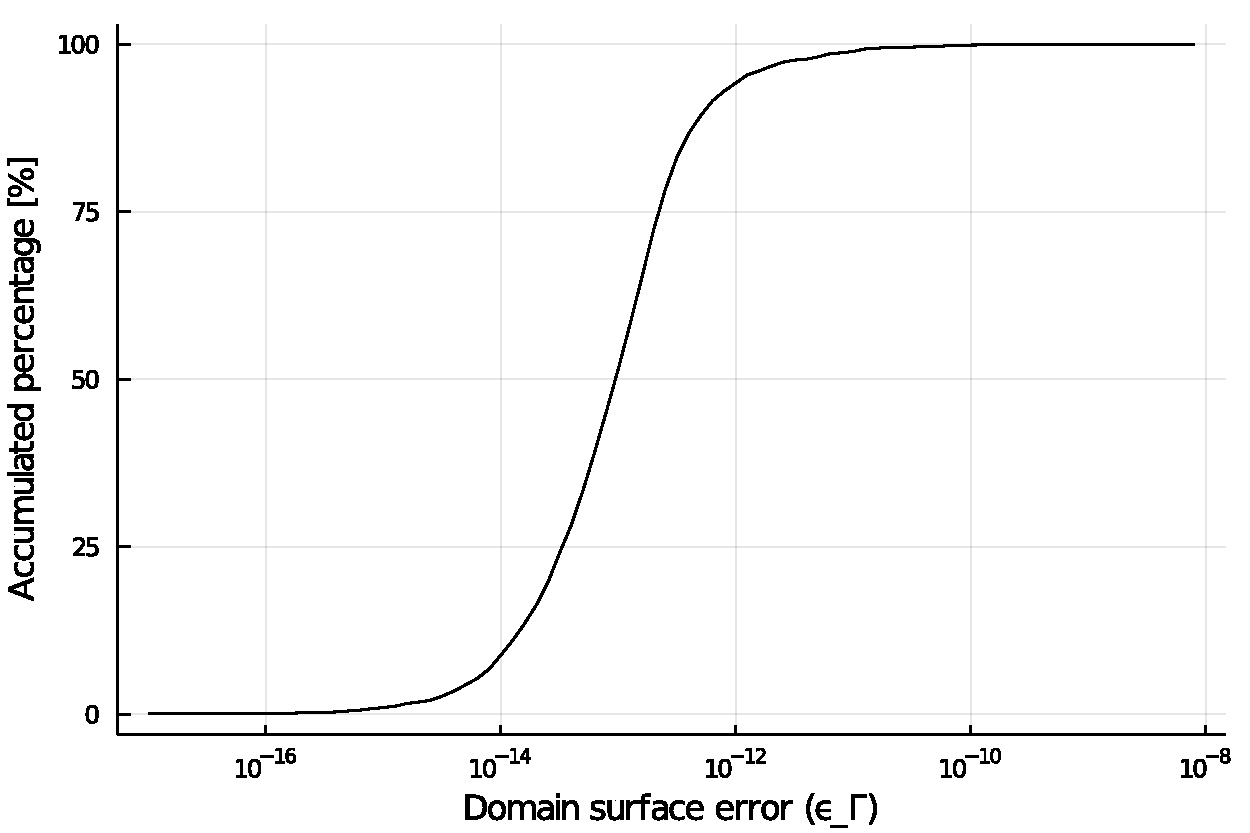
\includegraphics[width=0.49\textwidth]{../analysis/plots/filter_histogram_surface_error}
\end{frame}

\begin{frame}{Thingi 10k dataset}

  \begin{block}{CPU time}
  \begin{itemize}
    \item
      Not precise measure (different machines, single runs)
    \item
      Increasing with the number of STL facets
  \end{itemize}
  \end{block}

  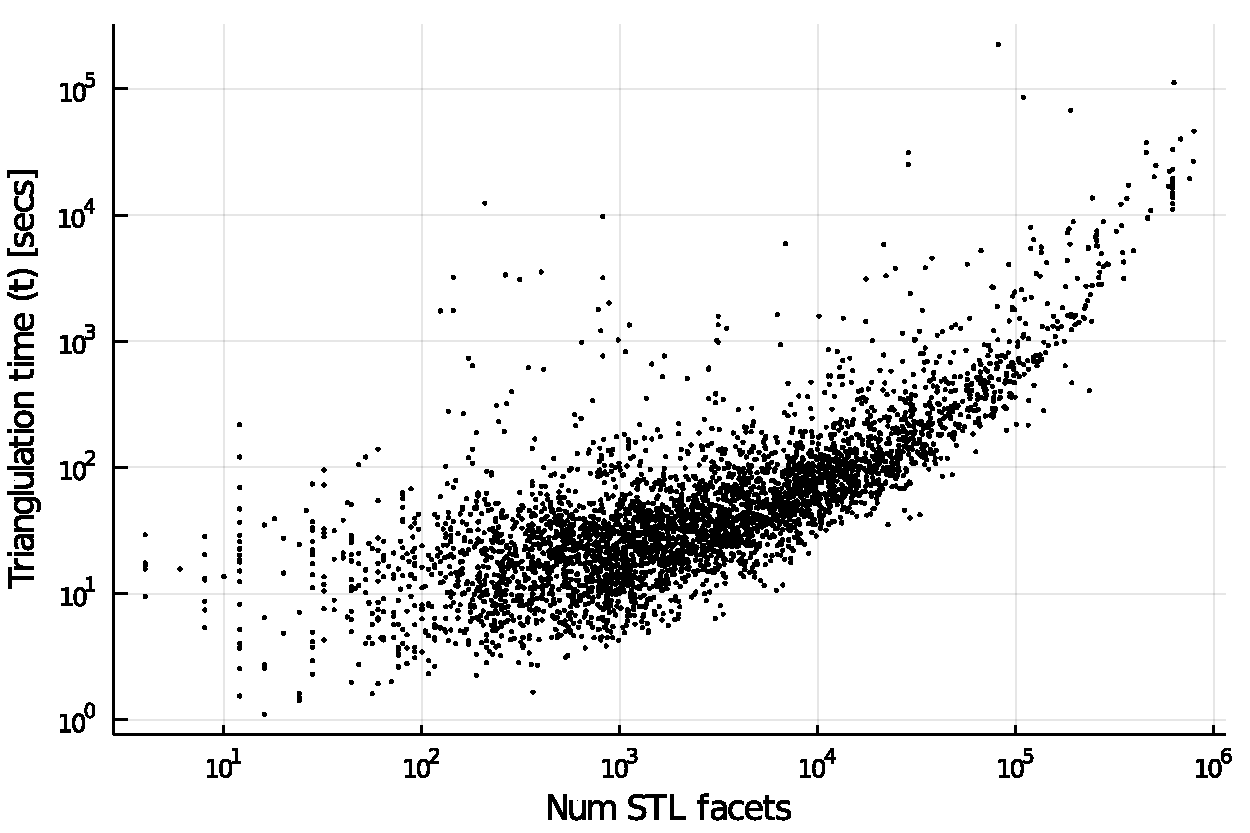
\includegraphics[width=0.49\textwidth]{../analysis/plots/num_stl_facets_time}
  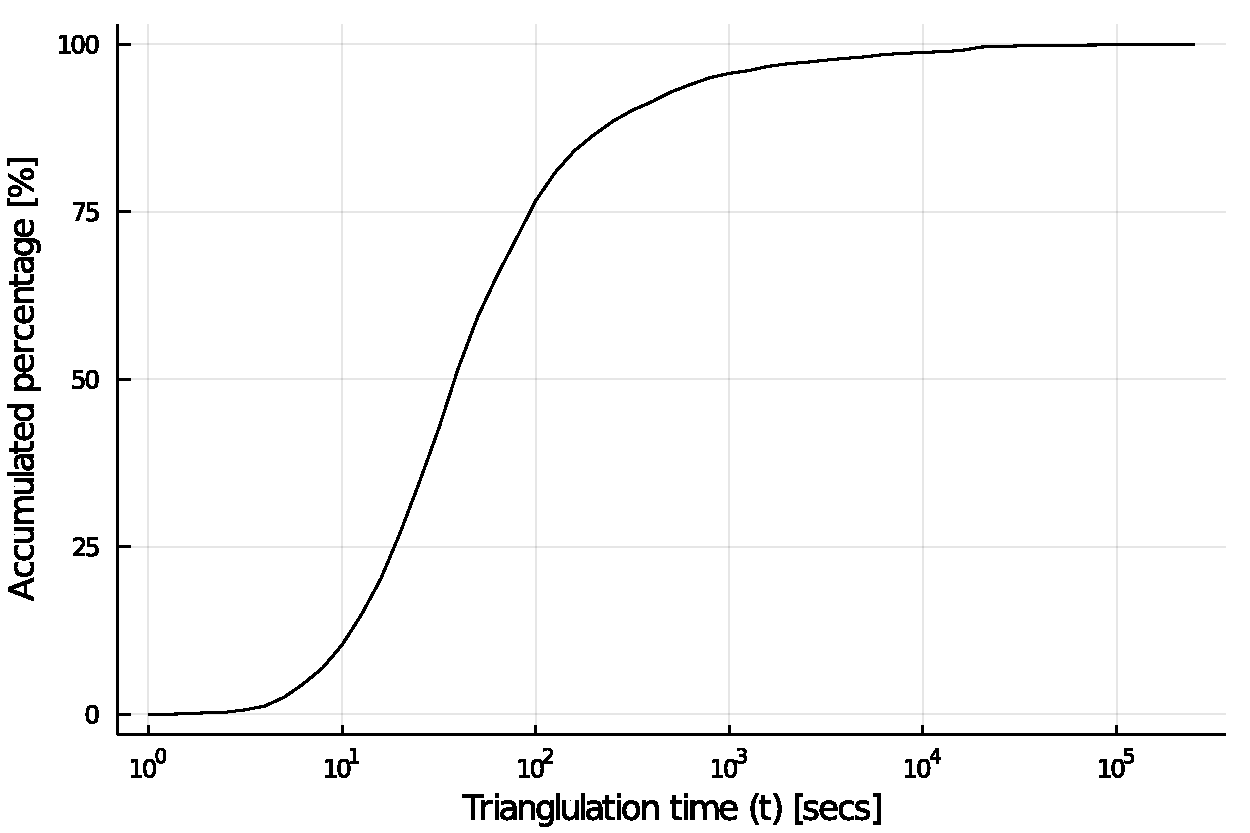
\includegraphics[width=0.49\textwidth]{../analysis/plots/histogram_time}
\end{frame}


\begin{frame}{Robustness matrix}
  \framesubtitle{Summary}

  \textbf{100\%} of ended test have volume and surface error bounded 
  ($\epsilon_{vol} < 10^{-14}$,$\epsilon_{surf} < 10^{-12}$) 

  \begin{block}

  The mesh sizes have $n_{max}$ multiple of 14 as the bounding box is expanded 
  a factor $0.2$ in each direction, thus the domain is 1.4 times the 
  bounding box per axis. The background cells will match the STL bounding box, 
  stressing even more the algorithm.
  \end{block}

  \vfill{}
  NOTE: Due to large computational requirements (time/memory),
  some tests have not ended.
  Those points are missing at the lowest and largest sizes.
  \begin{itemize}
    \item
      Low $n_{max}$: large amount of STL facets per cell
    \item
      High $n_{max}$: large background mesh

  \end{itemize}
 

\end{frame}


%\begin{frame}{Robustness matrix}
%  
%  \textbf{Collected results:}
%
%  \begin{itemize}
%    \item  
%      \href{run:domain_volume.pdf}{Domain Volume Variation}
%    \item
%      \href{run:domain_surface.pdf}{Domain Surface Variation}
%    \item
%      \href{run:volume_error.pdf}{Domain Volume Error}
%    \item
%      \href{run:surface_error.pdf}{Surface Error}
%    \item
%      \href{run:time.pdf}{CPU time (not accurate)}
%    \item
%      \href{run:subcells_x_cell.pdf}{\{Min,Max,Avg\} num subcells per cell }
%  \end{itemize}
%
%
%\end{frame}


\begin{frame}{Conclusions and pending work}

  \textbf{Conclusion so far}
  \begin{itemize}
    \item
      Issues are depending on the geometry
    \item
      Most of problematic geometries can be found \textit{a priori}
  \end{itemize}
  \textbf{Ongoing work}
  \begin{itemize}
    \item
      Detect true degenerated geometries
    \item
      Run Gridap
  \end{itemize}


\end{frame}
\end{document}
